\chapter{Experiments and Results}
\label{cha:ResearchAndResults}

The main goal of this work was to use machine learning algorithms to identify individuals with lung cancer from their circulating miRNA contents. This chapter describes the experiments done toward this goal. Specifically, I present the studies included in the experiments (\autoref{sec:res_studies_included}), investigate pairwise correlation in case-control differences between the studies (\autoref{sec:res_log_fold_change}), evaluate to what extent there is evidence for individual miRNAs are consistently differentially expressed across studies (\autoref{sec:res_evidence_consistently_differentially}), find to what extent machine learning algorithms can distinguish samples from different datasets (\autoref{sec:res_datasets_separable}), find a hierarchical clustering of the datasets based on their differential expression in miRNAs between cases and controls (\autoref{sec:res_hierarchical_clustering}), do machine learning on case-control status internally in each dataset (\autoref{sec:res_machine_learning_single}), find a single miRNA-sequence to use as baseline across datasets (\autoref{sec:baseline_miRNA_res}), find if any principal components in the biggest datasets have any association with case-control status (\autoref{sec:res_pca_analysis}), do machine learning across different datasets (\autoref{sec:res_machine_learning_multiple}), group datasets based on characteristics and do machine learning in each group (\autoref{sec:res_stratification}), find whether the largest principal components are noise and whether their removal is beneficial (\autoref{sec:pca_remove_artifacts_res}), find whether an RPM threshold for miRNAs in sequencing datasets is beneficial (\autoref{sec:res_rpm_threshold}), explore whether samples are contaminated by red blood cells (\autoref{sec:res_red_blood_cells}), create a web application for visualizing the data (\autoref{sec:res_web_application}) and do some further exploration based on the visualizations in the web application (\autoref{sec:res_results_from_web}).

\section{Studies included}
\label{sec:res_studies_included}
Current literature is replete with studies investigating the potential of circulating miRNAs for lung cancer diagnosis, but for such studies to be useful for machine learning analyses and for replication purposes, the data from individual miRNAs and individuals should be available. To identify a large and unbiased set of studies that had investigated and reported the blood expression profiles of multiple miRNAs in multiple individuals, including both lung cancer patients and controls, I did a structured literature review (see \autoref{sec:literature_review}). 

The review identified 123 studies. However, most datasets that were requested by email were not received. The 26 studies whose datasets that were either received or were publicly available are: \py{", ".join(f"\\citet{{{study}}}" + ("\\footnote{\\citet{Chen2019} is not the study where the dataset originated from, but it is a study using the dataset. The dataset is GSE71661 in the Gene Expression Omnibus, and has no citation listed: \\url{https://www.ncbi.nlm.nih.gov/geo/query/acc.cgi?acc=GSE71661}}" if study == "Chen2019" else "") for study in studies)}. A basic overview of the different studies is found in \autoref{tab:studies}. A more detailed overview of the studies is found in \citet{forprosjekt}\footnote{\citet{Abdollahi2019} is not described in \citet{forprosjekt} as the data was received too late for it to be included.}.

\sisetup{round-mode=places, round-precision=3}
\begin{sidewaystable}
    \caption{Characteristics of the studies in this project. The columns are as follows: \textit{Study}: The study the row is describing, \textit{Technology}: The technology used to measure miRNA in that study, \textit{Blood fraction}: What blood fraction is used for measuring miRNAs, \textit{\# miRNAs}: The number of different miRNA-sequences that are measured in the study, \textit{\# Cases}: The number of samples from cancer patients in the study, \textit{\# Controls}: The number of healthy controls in the study, \textit{Total}: The total number of samples in the study. EV = Extracellular Vehichle, Ex = Exsomal}
    \label{tab:studies}
    \resizebox{\textwidth}{!}{
        \csvreader[head to column names, tabular=|r|c|c|c|c|c|c|, table head=\hline \bfseries Study & \bfseries Technology & \bfseries Blood fraction & \bfseries \# miRNAs & \bfseries \# Cases & \bfseries \# Controls & \bfseries \# Total \\\hline, late after line=\\, late after last line=\\\hline]{tables/study_table.csv}{}{
            \citet{\csvcoli} & \csvcolii & \csvcoliii & \csvcoliv & \csvcolv & \csvcolvi & \csvcolvii
        }
    }
\end{sidewaystable}

\section{Log fold change correlation}
\label{sec:res_log_fold_change}
\citet{forprosjekt} showed that there is little log fold change correlation in the data. Furthermore, it showed that even though the correlation direction was arbitrary, there was a significant correlation between the datasets. However, the significance of the correlation was similar when randomizing the column corresponding to case-control, which means that the correlation could partially be a result of the covariance between different miRNA-sequences rather than due to case-control characteristics. The lack of correlation could be due to the characteristics of the different studies, in particular technology used and what blood fraction is measured. Therefore, a relevant experiment would be to see whether there is a larger correlation between datasets using the same technology and blood fraction, contrasted with the correlation when the datasets differ in these characteristics.

Due to the limited amount of datasets in this project, grouping based on both characteristics would give too low statistical power to make any conclusions. Therefore, I will first group by technology and group by blood fraction afterward. I will use a t-test between the calculated correlations when both datasets are in the same category, to the correlation when only one of the datasets is in a certain group. To avoid spurious correlations, only pairs of datasets with at least 10 miRNAs in common are considered. The correlation is calculated using Pearson's r.

The results from when checking the log fold change correlation when comparing the datasets where both datasets are in the same category (the in-group), contrasted with when only one of the datasets is in the category (the out-group), are shown in \autoref{tab:log_fold_change_corr}. There was no significant change between the in-groups and the out-groups in any of the cases if one adjust for multiple testing. This might be due to a lack of statistical power as there are few datasets in this project. That said, regardless of the significance, the mean correlation is low. One should also note that, according to \citet{forprosjekt}, the correlation seemed to be due to covariance between miRNA expressions rather than due to case-control characteristics. Therefore, I will replicate the case-control randomization done in \citet{forprosjekt}, but only for the in-groups.

\begin{table}
    \caption{Pearson's r of the log fold change between pairs of datasets. The first column is what group of datasets is selected. The second column is the mean log fold change correlation for pairs of datasets inside the group. The third column is the mean log fold change correlation for pairs of datasets where one of the datasets is inside the group and the other dataset is outside the group. The fourth and the fifth columns are the result of a t-test where the correlation coefficients in the in-group and the out-group were compared, with the t-statistic and the corresponding two-sided p-value.\\ Note: IG = in-group, OG = out-group}
    \label{tab:log_fold_change_corr}
    \sisetup{round-mode=places, round-precision=3}
    \begin{center}
        \csvreader[head to column names, tabular=|r|c|c|c|c|,
        table head = \hline \bfseries Group & \bfseries Mean IG & \bfseries Mean OG & \bfseries t-value & \bfseries p-value \\\hline,
        late after line=\\, late after last line=\\\hline]{tables/LogFoldChange/log_fold_change_corr_strat.csv}{}{
            \csvcoli & \num{\csvcolii} & \num{\csvcoliv} & \num{\csvcolvi} & \num{\csvcolvii}
        }
    \end{center}
\end{table}

The results from randomly assigning case-control status, and then calculating the pairwise log fold change correlation are shown in \autoref{tab:log_fold_change_corr_rand}. As there is no significant difference in the correlations, it seems that there was no significant correlation that could be separated from the effect of covariance between the miRNAs. There is a difference between the experiment done here and the experiment in \citet{forprosjekt}, namely that here I look at the direction of the correlation, while \citeauthor{forprosjekt} primarily looked at the significance of the correlation. It might be that the case-control characteristics are the cause of the direction of the correlation, whilst covariance between the miRNA-sequences is the cause of the significance of the correlation.

\begin{table}
    \caption{Pearson's r of the log fold change between pairs of datasets inside each group when case-control status is shuffled and not shuffled. The first column is what group of datasets is analyzed for the row. The second column is the mean log fold change correlation coefficient when the case-control characteristics are not shuffled. The third column is the mean log fold change correlation coefficient when the case-control characteristics are shuffled. The fourth and fifth columns are the result of a t-test where the correlation coefficients are compared when shuffled and when not shuffled, with the corresponding t-value and a two-sided p-value}
    \label{tab:log_fold_change_corr_rand}
    \resizebox*{\textwidth}{!}{
    \sisetup{round-mode=places, round-precision=3}
        \csvreader[head to column names, tabular=|r|c|c|c|c|,
        table head = \hline \bfseries Group & \bfseries Mean Non-shuffled & \bfseries Mean Shuffled & \bfseries t-value & \bfseries p-value \\\hline,
        late after line=\\, late after last line=\\\hline]{tables/LogFoldChange/log_fold_change_corr_strat_rand.csv}{}{
            \csvcoli & \num{\csvcolii} & \num{\csvcoliv} & \num{\csvcolvi} & \num{\csvcolvii}
        }}
\end{table}

It is hard to test the last hypothesis as the p-values do not have a known distribution. They are not uniformly distributed as there is a significant correlation between the datasets. They are also far from normally distributed, due to a very strong left skew, which would make a t-test give misleading results. One possibility might be to log-transform the p-values. The results are shown in \autoref{fig:log_fold_pvalue_log}. Neither are normally distributed, but the distribution of the log-transformed p-values seems closer to a normal distribution than the non-transformed p-values. 

\begin{figure}
    \begin{subfigure}[b]{0.5\textwidth}
        \resizebox{\textwidth}{!}{
            \begin{tikzpicture}
                \begin{axis}[
                        xlabel={p-values},
                        ylabel={Count},
                        ybar,
                        ymin=0
                    ]
                    \addplot[
                        hist = {
                            bins=40,
                            data min=0,
                            data max=1
                        },
                        table/col sep=comma,
                        fill=blue
                    ]
                    table[y={p-values}]{tables/LogFoldChange/log_fold_change_corr_strat_pvalue_log.csv};
                \end{axis}
            \end{tikzpicture}
        }
        \caption{Non-transformed}
        \label{fig:log_fold_pvalue_log_nt}
    \end{subfigure}
    \begin{subfigure}[b]{0.5\textwidth}
        \resizebox{\textwidth}{!}{
            \begin{tikzpicture}
                \begin{axis}[
                        xlabel={p-values (log)},
                        ylabel={Count},
                        ybar,
                        ymin=0
                    ]
                    \addplot[
                        hist = {
                            bins=40,
                            data min=-15,
                            data max=1
                        },
                        table/col sep=comma,
                        fill=blue
                    ]
                    table[y={log p-values}]{tables/LogFoldChange/log_fold_change_corr_strat_pvalue_log.csv};
                \end{axis}
            \end{tikzpicture}
        }
        \caption{Log-transformed}
        \label{fig:log_fold_pvalue_log_t}
    \end{subfigure}
    \caption{p-values of the log-fold-change correlation between each pair of studies with the same technology or the same body fluid}
    \label{fig:log_fold_pvalue_log}
\end{figure}

\begin{pycode}
df = pd.read_csv("tables/LogFoldChange/log_fold_change_corr_strat_pvalue_diff.csv")
\end{pycode}

The experiment thus becomes to look at the log transformed p-values when randomizing the case-control assignment and the log transformed p-values without randomization. Then a t-test will be performed to check for a possible difference in the p-values between the randomized and the non-randomized case. The t-test showed that the correlation was more significant when the case-control assignment was not randomized (\py{"$p=%.3f$" % df["p-value"]}), which suggests that case-control characteristics are the cause of some of the significance in the correlations, rather than it being only due to covariance between miRNA expressions.

None of the differences in \autoref{tab:log_fold_change_corr} were significant. It might be that some of the differences would be significant with more statistical power. One possible test is to test all correlations that are in in-groups to all correlations that are only in out-groups. This would have more statistical power, with the disadvantage that it does not say anything about which groups have more internal consistency, as it seems like it varies between the groups.

\begin{pycode}
df = pd.read_csv("tables/LogFoldChange/log_fold_change_corr_strat_all.csv")
\end{pycode}
The result was that there was still no significant difference between the in-groups and the out-groups when aggregating over all categories (\py{"$p=%.3f$" % df["p-value"]}), which suggests that the increased correlation in in-groups is either non-existent or too small to be found with the current number of datasets. Either way, the mean correlation in the in-group was \py{"$r=%.3f$" % df["mean IG"]}, which is a very small correlation that would suggest that case-control characteristics' effect on log fold change is either much smaller than the other effects, or the effects cannot be replicated across datasets. Indeed, \citet{forprosjekt} shows using linear regression that the proportion of variance in the miRNA expression that is due to case-control characteristics varies and is generally quite small. The highest proportion is $0.446$ in \citet{Duan2021} and the smallest is $0.009$ in \citet{Leidinger2014}. The proportion found by linear regression is probably overstating the actual proportion due to overfitting to the data, as the proportion of explained variance was smaller in datasets with larger sample sizes \citep{forprosjekt}.

\subsection{Using stages}
There is some evidence that suggests that the diagnostic accuracy of microRNA is somewhat higher in later stages of lung cancer \citep{later_better}. Thus, it might be valuable to check whether there is a higher log fold change correlation when only using cancer samples with advanced stages, in this case, stage 3 and 4. The log fold change is in this case  the difference between the mean expression in the cancer samples in advanced stages and the controls. If the correlation is better when considering later stages, that might suggest that later stages have more consistent expression, and thus are easier to diagnose. The test will be a t-test of the correlation coefficients when only stage 3 and 4 are considered, compared to the correlation coefficients when only stage 1 and 2 are considered.

The datasets where stage is marked are \citet{Abdollahi2019,Bianchi2011,Zaporozhchenko2018,Duan2021,Boeri2011,Leidinger2011,Qu2017,Li2017,Nigita2018}. However, \citet{Duan2021} only have samples in stages 1 and 2, and is therefore not used in this analysis. The results when only using advanced stages or only using early stages are shown in \autoref{tab:log_fold_stages}. This shows that there is no significant difference in the log fold change correlation when only considering late stages compared to when only considering early stages. The sample size is small, though, which makes it hard to conclude anything with certainty. However, the results suggest that there is no large improvement in log fold change correlation when using only late stage cancer, and if anything the correlation is higher in earlier stages. Indeed, \citet{later_better} suggested that the improvement in the diagnostic value of miRNA in late stage cancer was relatively small.


\begin{table}
    \caption{Pearson's r of the log fold change between pairs of datasets when only stages 3 and 4 are considered compared to when only stages 1 and 2 are considered, and the result from a t-test between the early and late stage log fold change correlation coefficients, with a t-value and a two-sided p-value.}
    \label{tab:log_fold_stages}
    \sisetup{round-mode=places, round-precision=3}
    \begin{center}
        \csvreader[head to column names, tabular=|c|c|c|c|,
        table head = \hline \bfseries Mean Late & \bfseries Mean Early & \bfseries t-value & \bfseries p-value \\\hline,
        late after line=\\, late after last line=\\\hline]{tables/LogFoldChange/log_fold_change_correlation_late.csv}{}{
            \num{\csvcoli} & \num{\csvcoliii} & \num{\csvcolv} & \num{\csvcolvi}
        }
    \end{center}
\end{table}



\section{Evidence for consistently differentially expressed miRNA-sequences}
\label{sec:res_evidence_consistently_differentially}
One question that has to be considered, especially given how \citet{forprosjekt} found that sign of the log fold change correlation was virtually arbitrary, is whether there is evidence that there exists any consistently differentially expressed miRNA-sequences at all. By consistently, I mean that it is differentially expressed in the same direction (up- or down-regulated) across studies. \Autoref{sec:baseline_miRNA_res} shows that some miRNA-sequences are often differentially expressed, but that the direction is not consistent, which would make diagnosis hard and lead one to question whether the differential expression was primarily due to case-control characteristics. It is difficult to rule out that there exist any consistently differentially expressed miRNA-sequences, especially as many of the miRNA-sequences are only present in a few datasets, which would mean that it would be hard to say whether the differential expression is due to chance or study characteristics, or if it is due to case-control characteristics.

\subsection{Paired sign test}
\label{subsec:paired_sign_test_res}

\begin{pycode}
df = pd.read_csv("tables/ConsistentExpression/mirna_consistent_expression.csv", index_col=0)
prob = round((1 - df.loc["Both significant", "probability"])*100)
\end{pycode}
The calculated probabilities that a miRNA-sequence is differentially expressed in the same way in two different studies are shown in \autoref{tab:evidence_res}, where the pairs are filtered on whether the differential expression is statistically significant in the different studies. The experiment is described in more detail in \autoref{subsec:paired_sign_test_met}. None of the probabilities are higher than $0.50$, which suggests that there is no consistency in the differential expression of single miRNAs. However, there is still a need to check if there is a confounder in the technology or blood fraction used in the different studies.

\iffalse
which gives evidence that there are miRNA-sequences that have a differential expression that have a differential expression that is more consistent than chance levels. Especially the case when only considering pairs when both were significant one achieves a probability that is somewhat better than chance. On one hand, this suggests that there are some consistencies between datasets, which could mean that there might be possible to find a model that diagnose better than chance across datasets. On the other hand, in \py{f"${prob}\\%$"} of the cases there are inconsistencies in the direction of differential expression of the miRNA-sequences. One problem is that this would limit the results from naïve machine learning, as a machine learning algorithm might find one miRNA to be a good separator in one dataset, and if this miRNA is differentially expressed in the test dataset, there is a \py{f"{prob}\\%"} chance that the miRNA-sequence will separate the cases and controls in the wrong way! One important question that arises is why this happens in the pairs where both are significant?
\fi


\begin{table}
    \caption{The results from an experiment where one takes a pair of datasets that have measured the same miRNA. Then one checks whether the signs of the fold change are equal or not equal. The first column is what pairs are used, where significant means the log fold change was significantly different from zero using a two-sided t-test and a significance level of $0.05$. One or both refers to whether the differential expression was significant in one or both datasets in the pair. The second column is the portion of the pairs that have the same sign, or if you know the sign of one of the datasets in the pair, then it is the probability that the other pair has the same sign. Finally, the last column contains a p-value, which is the resulting p-value from a one-sided binomial test on whether the portion of pairs with the same sign is larger than $0.50$.}
    \label{tab:evidence_res}
    \sisetup{round-mode=places, round-precision=3}
    \begin{center}
        \csvreader[head to column names, tabular=|r|c|c|,
        table head = \hline \bfseries Pairs & \bfseries Probability & \bfseries p-value \\\hline,
        late after line=\\, late after last line=\\\hline]{tables/ConsistentExpression/mirna_consistent_expression.csv}{}{
            \csvcoli & \num{\csvcolii} & \num{\csvcoliii}
        }
    \end{center}
\end{table}

\subsubsection{Stratification of the datasets}
If the differences are due to technology or blood fraction, one might assume that the consistency is higher when only checking against datasets where these characteristics are similar. The results from an analysis checking only significant pairs where both studies share a characteristic is shown in \autoref{tab:evidence_res_strat}. Whole blood is the only group that gives significantly better than chance levels. Still, it was only slightly better than chance level, which suggests that neither technology nor body fluid is the cause of the poor consistency.

\begin{table}
    \caption{The results from an experiment where one takes pairs of datasets that share a certain characteristic and that have measured the same miRNA. Then one checks whether the signs of the fold change are equal or not equal, only using pairs where the log fold change was significantly different from zero, using a two-sided t-test. The first column is what characteristic the datasets in that row share. The second column is the portion of the pairs that have the same sign, or if you know the sign of one of the datasets in the pair, then it is the probability that the other pair has the same sign. Finally, the last column contains a p-value, which is the resulting p-value from a one-sided binomial test on whether the portion of pairs with the same sign is larger than $0.50$.}
    \label{tab:evidence_res_strat}
    \sisetup{round-mode=places, round-precision=3}
    \begin{center}
        \csvreader[head to column names, tabular=|r|c|c|,
        table head = \hline \bfseries Group & \bfseries Probability & \bfseries p-value \\\hline,
        late after line=\\, late after last line=\\\hline]{tables/ConsistentExpression/mirna_consistent_expression_strat.csv}{}{
            \csvcoli & \num{\csvcolii} & \num{\csvcoliii}
        }
    \end{center}
\end{table}

\subsubsection{Possible significance levels}
One issue that remains is the significance level. I sat a significance level of $p=0.05$, but if the number of miRNAs that are differentially expressed due to case-control characteristics is low, this will lead to a large portion of false positives among the miRNAs found to be significantly differentially expressed. Due to that, I tried with different significance levels, and the results are shown in \autoref{tab:evidence_res_pval}. There seems to be a general upward trend where a more stringent significance level results in a higher consistency. However, none of the significance levels result in a consistency significantly better than chance levels, and the highest probability is still only very slightly better than chance. Thus, the lack of consistency was not due to a high significance level or similarly a high share of false positives.

\begin{table}
    \caption{The results from an experiment where one takes a pair of datasets that have measured the same miRNA. Then one checks whether the signs of the fold change are equal or not equal. The first column is what pairs are used, where significant means the log fold change was significantly different from zero in both datasets using two-sided t-tests and the given significance level. The second column is the portion of the pairs that have the same sign, or if you know the sign of one of the datasets in the pair, then it is the probability that the other pair has the same sign. Finally, the last column contains a p-value, which is the resulting p-value from a one-sided binomial test on whether the portion of pairs with the same sign is larger than $0.50$}
    \label{tab:evidence_res_pval}
    \sisetup{round-mode=figures, round-precision=3}
    \begin{center}
        \csvreader[head to column names, tabular=|r|c|c|,
        table head = \hline \bfseries Significance level & \bfseries Probability & \bfseries p-value \\\hline,
        late after line=\\, late after last line=\\\hline]{tables/ConsistentExpression/mirna_consistent_expression_pvalues.csv}{}{
            \num[round-precision=1, exponent-mode=scientific]{\csvcoli} & \num{\csvcolii} & \num{\csvcoliii}
        }
    \end{center}
\end{table}

\subsection{Signed-rank test with cross validation}
Here are the results from the signed-rank test including when cross validation was used, which is another method to check for consistent differential expression in miRNA.

\subsubsection{Cross validation}
\label{subsubec:signed_rank_cv_res}

This is an experiment where a signed-rank test is used to find the most and least consistently differentially expressed miRNAs in a set of datasets, and then one uses two external datasets to see whether the consistency generalizes. The experiment is described in more detail in \autoref{subsubsec:met_signed_rank_cv}. The results are shown in \autoref{tab:signed_rank_cv}. The results suggest that the miRNA-sequences that were the most consistently differentially expressed in the signed-rank test were somewhat more consistently differentially expressed in the two excluded datasets. The difference is significant at a $0.05$-level, but there have been done many statistical tests in this chapter, and adjusted for this multiple testing it is not significant. What results in this poor consistency? One hint may lay in \autoref{subsec:paired_sign_test_res}, which suggests that the consistency in might be better if only looking at pairs where both are significantly differentially expressed.

\begin{table}
    \caption{The proportion of pairs that had the same direction of differential expression in the two excluded datasets, among the miRNAs that were shown to be most and least consistently differentially expressed in the signed-rank test as described in \autoref{subsubsec:met_signed_rank_cv}. The t-value is the t-value for the difference between the two proportions, and the p-value is the corresponding p-value.}
    \label{tab:signed_rank_cv}
    \sisetup{round-mode=figures, round-precision=3}
    \begin{center}
        \csvreader[head to column names, tabular=|c|c|c|c|c|c|c|c|,
        table head = \hline \bfseries Most significant & \bfseries Least significant & \bfseries t-value & \bfseries p-value \\\hline,
        late after line=\\, late after last line=\\\hline]{tables/SignedRank/signed_rank_cv.csv}{}{
            \num{\csvcoli}  & \num{\csvcoliii} & \num{\csvcolv} & \num{\csvcolvi}
        }
    \end{center}
\end{table}

\paragraph{Only pairs with significantly differentially expressed miRNAs} \mbox{} \\
Now I will only consider pairs where both are significantly differentially expressed in the two excluded datasets using a t-test and a significance level of $p = 0.05$. The results are shown \autoref{tab:signed_rank_cv_significant}. The results show that there is no significant difference in the proportion of the pairs with the same direction of differential expression. This suggests that the lack of improvement in the proportion in \autoref{subsubec:signed_rank_cv_res} was not the result of insignificance in the differential expression in the pairs.

\begin{table}
    \caption{The proportion of pairs that had the same direction of differential expression in the two excluded datasets, among the miRNAs that were shown to be most and least consistently differentially expressed in the signed-rank test as described in \autoref{subsubsec:met_signed_rank_cv}. The miRNA sequence had to be significantly differentially expressed in the two excluded datasets in a t-test. The t-value in the table is the t-value for the difference between the two proportions, and the p-value is the corresponding p-value.}
    \label{tab:signed_rank_cv_significant}
    \sisetup{round-mode=figures, round-precision=3}
    \begin{center}
        \csvreader[head to column names, tabular=|c|c|c|c|c|c|c|c|,
        table head = \hline \bfseries Most significant & \bfseries Least significant & \bfseries t-value & \bfseries p-value \\\hline,
        late after line=\\, late after last line=\\\hline]{tables/SignedRank/signed_rank_cv_significant.csv}{}{
            \num{\csvcoli}  & \num{\csvcoliii} & \num{\csvcolv} & \num{\csvcolvi}
        }
    \end{center}
\end{table}

\paragraph{Using t-test results instead of log fold change in signed-rank test} \mbox{} \\
One possible reason for the results in \autoref{subsubec:signed_rank_cv_res} could be that small studies have a big log fold change due to chance. Therefore, I will also try using t-test results in the signed-rank test as explained in \autoref{subsubsec:met_t_test_signed_rank}. The results are shown in \autoref{tab:signed_rank_cv_tvalue}. Neither here were there any signs of external validity in the results from the signed-rank test. Thus, either the signed-rank test is a subpar way to find what miRNAs are the most consistently differentially expressed, or there are no consistently differentially expressed miRNAs.

\begin{table}
    \caption{The proportion of pairs that had the same direction of differential expression in the two excluded datasets, among the miRNAs that were shown to be most and least consistently differentially expressed in the signed-rank test as described in \autoref{subsubsec:met_signed_rank_cv}, with the difference that the p-value of a t-test of the log fold change was used instead of the log fold change. The t-value in the table is the t-value for the difference between the two proportions, and the p-value is the corresponding p-value.}
    \label{tab:signed_rank_cv_tvalue}
    \sisetup{round-mode=figures, round-precision=3}
    \begin{center}
        \csvreader[head to column names, tabular=|c|c|c|c|c|c|c|c|,
        table head = \hline \bfseries Most significant & \bfseries Least significant & \bfseries t-value & \bfseries p-value \\\hline,
        late after line=\\, late after last line=\\\hline]{tables/SignedRank/signed_rank_cv_tvalue.csv}{}{
            \num{\csvcoli}  & \num{\csvcoliii} & \num{\csvcolv} & \num{\csvcolvi}
        }
    \end{center}
\end{table}

\subsubsection{Signed-rank test}
A signed-rank test was done using all datasets. The signed-rank test was done both using log fold change and using t-test results. Using t-test results is explained in \autoref{subsubsec:met_t_test_signed_rank}, and this experiment is explained in more detail in \autoref{subsubsec:met_singed_rank_no_cv}. The results are in \autoref{tab:signed_rank}. As \autoref{subsubec:signed_rank_cv_res} suggests that this test has low external validity, one should be careful when using this data for conclusions. None of the miRNA-sequences were significantly consistently differentially expressed in the datasets when adjusted for multiple testing, which could either be because there is no such miRNA-sequence, or there are too few datasets included in this study to get enough statistical power to find any.

\begin{table}
    \caption{The most consistently differentially expressed miRNA-sequences according to a signed-rank test as described in \autoref{subsubsec:met_singed_rank_no_cv}. p-values are adjusted using Bonferroni correction. The direction is whether the miRNA is up- or down-regulated in cancer. The headers of the subtables tell whether it is the log fold change or the results from t-tests that is the input to the signed-rank test}
    \label{tab:signed_rank}
    \sisetup{round-mode=figures, round-precision=3}
    \begin{subtable}[h]{0.5\textwidth}
        \caption{Using log fold change}
        \resizebox{\textwidth}{!}{
            \csvreader[head to column names, tabular=|r|c|c|,
                table head = \hline \bfseries MiRNA & \bfseries p-value & \bfseries Direction \\\hline,
                late after line=\\, late after last line=\\\hline]{tables/SignedRank/signed_rank.csv}{}{
                \csvcoli  & \num{\csvcolii} & \csvcoliii
            }
        }
    \end{subtable}
    \begin{subtable}[h]{0.5\textwidth}
        \caption{Using t-test results}
        \resizebox{\textwidth}{!}{
            \csvreader[head to column names, tabular=|r|c|c|,
                table head = \hline \bfseries MiRNA & \bfseries p-value & \bfseries Direction \\\hline,
                late after line=\\, late after last line=\\\hline]{tables/SignedRank/signed_rank.csv}{}{
                \csvcoliv  & \num{\csvcolv} & \csvcolvi
            }
        }
    \end{subtable}
\end{table}

\section{Are datasets separable from each other?}
\label{sec:res_datasets_separable}
\begin{pycode}
df = pd.read_csv("tables/separate_datasets.csv", index_col=0)
\end{pycode}
One question arises when the consistency between the datasets is as poor as it has been shown to be in \citet{forprosjekt}, namely can one recognize what dataset a sample is from? Given that there are differences between the datasets, can one use these differences to recognize a dataset? The way I will test this is using logistic regression on a pair of datasets where one-third of each dataset is used for testing and two-thirds is used for training. The model will be trained to separate samples from the two datasets from each other. Only pairs of datasets with at least 10 miRNA-sequences in common are considered. The metric to evaluate the separation is AUC.

Learning a logistic regression model to separate samples from two datasets lead to a mean AUC of \py{"$%.3f$" % df.loc["Logistic Regression", "mean"]} and a standard deviation of \py{"$%.3f$" % df.loc["Logistic Regression", "std"]}. The results were very poor, and somewhat suspicious, as a random separation would give an AUC of $0.50$. On the other hand, an AUC of \py{"$%.3f$" % df.loc["Logistic Regression", "mean"]} is good in some sense, because it separates well, but it mixes up the two categories. I do not know what caused this result, but there was strong evidence that the datasets could be separated, and therefore I tried using XGBoost instead. XGBoost gave a mean AUC of \py{"$%.3f$" % df.loc["XGBoost", "mean"]} with a standard deviation of \py{"$%.3f$" % df.loc["XGBoost", "std"]}. This suggests that the datasets can be separated from each other, but far from perfectly in general. However, looking at the AUC values, several had AUC $> 0.99$, which means that there were datasets that were easier to distinguish than others. One question that remains is whether this knowledge can be used to adjust the datasets so that they are more comparable. One possibility would be to use linear regression to find expression patterns that are characteristic of that dataset and then adjust for it. However, this would not work as the miRNA expressions are already standardized to a mean of $0$, so the linear regression would not find any mean effects of any dataset. Furthermore, logistic regression performed poorly compared to XGBoost when trying to separate datasets, which suggests that what distinguishes the datasets are non-linear patterns, which are hard to adjust for.

\section{Hierarchical clustering of datasets}
\label{sec:res_hierarchical_clustering}
\begin{pycode}
df1 = pd.read_csv("tables/Clustering/hierarchical_clustering_pairs.csv")
df2 = pd.read_csv("tables/Clustering/hierarchical_clustering_merged.csv")
\end{pycode}
Hierarchical clustering of miRNA expressions is a common analysis in this field. As I want to find patterns in the comparability of the datasets, I will try to cluster the datasets. This would not only give information about what datasets are more comparable, but also whether there are clusters of datasets that are closer to each other, and in that case, what characterizes them. This is somewhat similar to the analysis in \citet{forprosjekt} where \citeauthor{forprosjekt} created a graph of what datasets were similar. The difference is that the hierarchical clustering will give clusters of datasets that are similar to each other, rather than just comparing pairs of datasets.

The results from doing hierarchical clustering of the datasets are shown in \autoref{fig:hierarchical_clustering}. The clustering was based on the difference in log fold change as described in \autoref{sec:hierarchical_clustering_met}. There seem to be a close cluster that includes \citet{Wozniak2015,Leidinger2014,Patnaik2017,Leidinger2011,Keller2014}. It might be that these datasets are close to each other, and that models trained on one of the datasets would do well on the other datasets. Testing this hypothesis by training on pairs of datasets using logistic regression resulted in a mean AUC of \py{"$%.3f$" % df1["auc"].mean()} with a standard deviation of \py{"$%.3f$" % df1["auc"].std()}. Trying to test on one dataset while training on the others using XGBoost resulted in AUCs with a mean of \py{"$%.3f$" % df2["AUC"].mean()} and a standard deviation of \py{"$%.3f$" % df2["AUC"].std()}, which was not significantly higher than $0.500$, plausibly due to the low sample size. Overall, even though this is a cluster, the diagnostic value across these datasets is relatively low, at least compared to the internal diagnostic value found in \autoref{sec:machine_learning_single}.

\begin{figure}
    \centering
    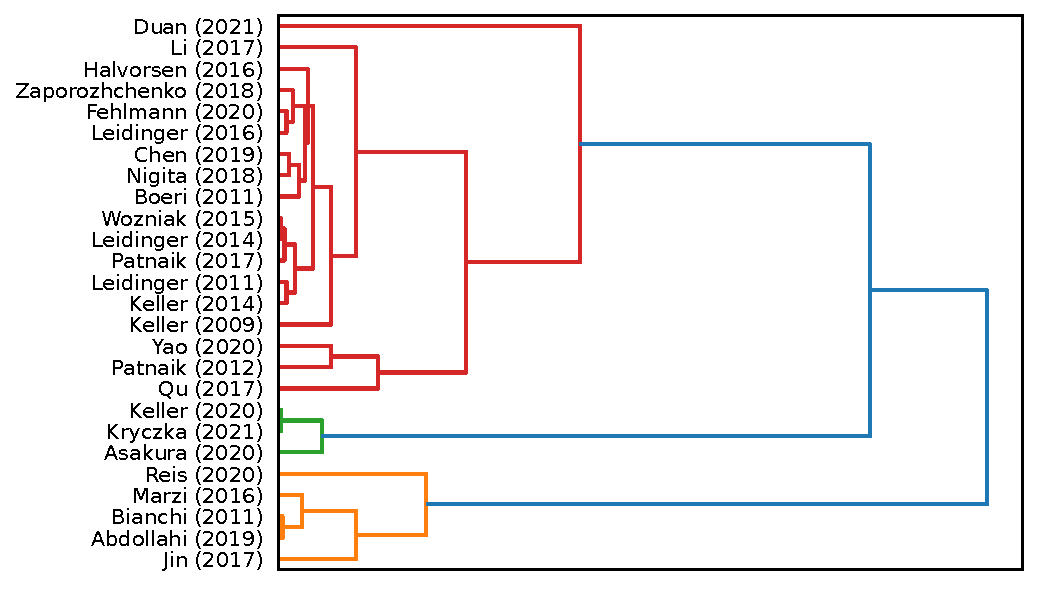
\includegraphics[width=\textwidth]{figs/hierarchical_clustering_datasets.pdf}
    \caption{Hierarchical clustering of the datasets, where the distance between the datasets is equal to the mean squared difference in log-fold-change. Coloring is for aesthetic reasons.}
    \label{fig:hierarchical_clustering}
\end{figure}

\section{Machine learning on single datasets}
\label{sec:res_machine_learning_single}
One question that was asked in \autoref{sec:Goals and Research Questions} was whether more advanced machine learning algorithms are better at diagnosing lung cancer based on miRNA-levels. Therefore, I have chosen to do machine learning on single datasets. As seen in \citet{forprosjekt}, the results when doing machine learning across datasets were mostly poor. Furthermore, if the connection between miRNA expression and lung cancer is very sensitive to study characteristics, machine learning across arbitrary different datasets might not be the best idea, compared to training on data where the characteristics are known to be the same. I have chosen four different types of machine learning algorithms to test.

\begin{itemize}
    \item Logistic regression: It is natural to use as a baseline model to compare against, as it has been used in many of the studies that are included in this project.
    \item Support vector machine: If the data are nearly linearly separable (which the PCA-plots in \citet{forprosjekt} suggest is often the case), this will find such a separation.
    \item Random forest: It is a powerful algorithm that is able to generalize well also on small datasets, as it is an ensemble method.
    \item XGBoost: Has had the most success in tabled data with limited samples in Kaggle competitions (see \autoref{subsec:xgboost}), and is thus a reasonable algorithm to test.
\end{itemize}

The results from machine learning on single datasets are shown in \autoref{tab:machine_learning_single}. The results are from using cross validation on the datasets with the given machine learning algorithms. A more detailed explanation is found in \autoref{sec:machine_learning_single}. Random forest performed best, while XGBoost performed worst. One question is whether these differences are statistically significant or not. Therefore, I performed t-tests on the differences in AUC values. The results are in \autoref{tab:machine_learning_single_pvalues}, which shows that none of the differences were significant. Thus one cannot say that one algorithm performed better than another in general.

\iffalse
There seem to be little difference in the overall results, except for  preforming somewhat worse than the other three, however the difference is small and the number of datasets is small. Therefore, XGBoost performing worse might be due to chance alone. No hyperparameter tuning was done, and hyperparameter tuning might would have changed the results somewhat, but overall it seems like the model used have little impact on the results. When looking at the results for a single dataset there is somewhat variance, but as the overall results are similar, the variance in results for a single dataset is likely the result of chance rather than intrinsic advantage of some models to some datasets. As the linear model, logistic regression, performs as well as non-linear models, SVM, random forest and XGBoost, there is limited evidence for non-linear relationships between miRNA expression and lung cancer. However, there might be that possible non-linear relationships are either too subtle to find at the current sample size, or the non-linear relationship might be a type that cannot be modelled with random forest or XGBoost. 
\fi


\begin{table}
    \caption{The mean AUC when using cross validation on the given studies with the given models, as described in \autoref{sec:machine_learning_single}. The first column says which dataset is used, and the rest of the columns have a column name that represents the model used. LR = Logistic Regression, RF = Random Forest}
    \label{tab:machine_learning_single}
    \centering
\begin{pycode}
df = pd.read_csv("tables/machine_learning_single.csv")
print("\\begin{tabular}{|r|c|c|c|c|}")
print("\\hline")
print("\\bfseries " + " & \\bfseries ".join(map(lambda x: x.replace("Logistic Regression", "LR").replace("Random Forest", "RF"), df.columns)))
for ind, row in df.iterrows():
    print(f"\\\\ {chr(92)+'hline' if ind == 0 else ''} \\citet{{{row['Study']}}}")
    row = row[1:]
    for r in row:
        print(" & ")
        print(f"\\cellcolor{{{'caribbeangreen' if r == max(row) else 'candypink' if r == min(row) else 'mygray'}}}")
        print("$%.3f$" % r)
print("\\\\ \\hline")
print("Mean & " + " & ".join("$%.3f$" % r for r in df.iloc[:, 1:].mean()))
print("\\\\ \\hline")
print("\\end{tabular}")
\end{pycode}
\end{table}

\begin{table}
    \caption{The p-values of the difference in mean AUC in \autoref{tab:machine_learning_single} using a two-sided t-test. The row and column labels represent what algorithms we are comparing. LR = Logistic Regression, RF = Random Forest}
    \label{tab:machine_learning_single_pvalues}
    \centering
\begin{pycode}
from scipy.stats import ttest_ind
df = pd.read_csv("tables/machine_learning_single.csv", index_col=0)
print("\\begin{tabular}{|r|c|c|c|c|}")
print("\\hline")
columns = list(map(lambda x: x.replace("Logistic Regression", "LR").replace("Random Forest", "RF"), df.columns))
print(" & \\bfseries " + " & \\bfseries ".join(columns))
for c1, c2 in zip(columns, df.columns):
    print(r"\\\hline")
    print(f"\\bfseries {c1}")
    for c3 in df.columns:
        print(" & ")
        if c2 == c3:
            continue
        print("$%.3f$ " % ttest_ind(df[c2], df[c3]).pvalue)
print(r"\\\hline")
print(r"\end{tabular}")
\end{pycode}
\end{table}

\subsection{Using stages}
Another question is whether there is any difference in AUC between early and late stage cancer. Therefore, I will train and test a logistic regression classifier on datasets where stage is labeled, using either only late stage cancer or only early stage cancer. The training and testing will follow the same cross validation strategy as above. The resulting AUCs when training and testing a logistic regression model on only late stage cancer or only on early stage cancer are shown in \autoref{tab:machine_learning_single_stages}. The results might suggest that there might be a higher AUC when only using late stage cancer, however, the statistical power here is too small to conclude with any certainty.

\begin{table}
    \caption{The mean AUC when using cross validation on the given studies when only using early stage cancer samples or only using late stage cancer samples. Empty fields mean that there were less than two cancer samples in the dataset, thus any inference would be impossible.}
    \label{tab:machine_learning_single_stages}
    \centering
\begin{pycode}
df = pd.read_csv("tables/Stratification/auc_stages_internal.csv")
print("\\begin{tabular}{|r|c|c|}")
print("\\hline")
print("\\bfseries " + " & \\bfseries ".join(df.columns))
for ind, row in df.iterrows():
    print(f"\\\\ {chr(92)+'hline' if ind == 0 else ''} \\citet{{{row['Study']}}}")
    row = list(row[1:])
    for r in row:
        print(" & ")
        print(f"\\cellcolor{{{'caribbeangreen' if r == np.max(row) else 'candypink' if r == np.min(row) else 'mygray'}}}")
        print("$%.3f$" % r if not np.isnan(r) else "*")
print("\\\\ \\hline")
print("Mean & " + " & ".join("$%.3f$" % r for r in df.iloc[:, 1:].mean()))
print("\\\\ \\hline")
print("\\end{tabular}")
\end{pycode}

\end{table}

\section{Baseline miRNA-sequence}
\label{sec:baseline_miRNA_res}
One question, as asked in \autoref{sec:Goals and Research Questions}, was what miRNA-sequences would be most successful in diagnosing lung cancer. This has not only clinical relevance, but is also important to have as a comparison for a machine learning model, as a complicated machine learning model would be worthless if one single miRNA-sequence had the same diagnostic value. In addition, there will always be additional costs associated with measuring more miRNA-sequences in a blood test, therefore ideally one would like to find the simplest model possible.

There are two main types of methods possible for finding such miRNA-sequences, each with some pros and cons:
\begin{enumerate}
    \item Look at meta-analyses for finding miRNA-sequences that are found to diagnose lung cancer well across studies. \\\\
        Pros:
        \begin{itemize}
            \item The miRNA-sequences found would be based on more data, and thus they are likely better.
            \item The miRNA-sequences are nearly\footnote{After all, the meta-analyses might be based on some datasets used in this project} independent of the datasets used in this project, and are therefore mostly unbiased.
        \end{itemize}
        Cons:
        \begin{itemize}
            \item The miRNA-sequences that are reported in these meta-analyses are often not in many of the datasets used in this project.
        \end{itemize}
    \item Look at the datasets used in this project to find miRNA-sequences that can separate cases and controls across the different datasets. \\\\
        Pros:
        \begin{itemize}
            \item It is easier to limit the search to miRNA-sequences that are found in many of the datasets in this project.
        \end{itemize}
        Cons:
        \begin{itemize}
            \item The miRNA-sequences are biased, as the baseline is the ability of these miRNA-sequences to diagnose cancer on the datasets, but the miRNA-sequences were chosen because they diagnosed well on said datasets.
        \end{itemize}
\end{enumerate}

I want to try a hybrid strategy, in order to mitigate the cons of each method. That is, I want to try to find an intersection between microRNA-sequences that have been found in meta-analyses to be consistently good at diagnosing lung cancer and microRNA-sequences that separate well in the studies used in this project.

There are several ways to measure to which degree a miRNA-sequence can be used to separate cases from controls. One possibility would be to use the t-statistic. The advantage of the t-statistic is that it has a known distribution (given the null hypothesis), and thus one could get to know whether a difference is plausibly a result of chance or not. The disadvantage of the t-statistic is that it does not only measure to which degree the miRNA-sequence separates well in the dataset, but also the statistical power of each dataset. Therefore, large datasets would be given more weight, and the value could hide to what degree the miRNA-sequence diagnoses correctly in the dataset.

Another alternative is to use Cohen's d. The advantage of Cohen's d is that it tells to what degree cases and controls are separated independently of the number of samples in the dataset. The disadvantage of Cohen's d is that it does not consider the statistical power at all, and thus one might expect a number of spurious results when using Cohen's d. A final statistic is to use AUC. The advantages and disadvantages are similar to Cohen's d, with the difference that AUC has the advantage that it is the metric that the results will be measured against in the end. However, Cohen's d has the advantage that it also looks at the size of the difference in expression, and not just whether there is a separation like AUC does.

After consideration of the different statistics, I found that Cohen's d and AUC will be the most appropriate statistic for this purpose, as the t-statistic would give too much power to the large datasets (which might not be representative at all) and not tell the actual degree of separation.

\subsection{Meta-analyses}
\label{subsec:meta_analyses}
Meta-analyses gave an overview of the possible miRNA-sequences that can be used as baselines in this project \citep{mirna_replicate_sequences,meta-mirna-2,meta-mirna-3,meta-mirna-4}, whereas \citet{mirna_replicate_sequences} was the most thorough of the meta-analyses. These meta-analyses suggest that the miRNA-sequences that have been shown to be able to diagnose lung cancer in the most studies are miR-21 and miR-210, with \citet{mirna_replicate_sequences} suggesting that miR-182, miR-155 and miR-17 are in third, fourth and fifth place, respectively. All of these miRNA-sequences were reported to be up-regulated in cases compared to controls. However, these results were not representative of the studies used in this project. 

\citet{mirna_replicate_sequences} found that of all studies that they went through miR-21 was significantly up-regulated in cases in 48 studies, and down-regulated in two studies. However, among the studies used in this project, \citet{Patnaik2012,Jin2017,Leidinger2016,Fehlmann2020} all reported that miR-21 was down-regulated in cases compared to controls, which suggests that miR-21 might not be as good of a biomarker for lung cancer as the meta-analyses suggest. An overview of the reported up- and down-regulation of the aforementioned miRNA-sequences in the studies in this project is shown in \autoref{tab:meta_mirna}. 

\newcommand{\colorupdown}[1]{
    \ifthenelse{\equal{#1}{Up}}{
        \cellcolor{caribbeangreen}
    }{
        \ifthenelse{\equal{#1}{Down}}{\cellcolor{candypink}}{\cellcolor{mygray}}
    }
    #1
}
\begin{table}
    \caption{Whether the miRNA-sequences were reported to be significantly up- or down-regulated ($p < 0.05$) in the studies. \\
    Note: \citet{Reis2020} only report miR-210 and miR-182 to be up-regulated in adenocarcinoma. In \citet{Wozniak2015} and \citet{Keller2014} abu-miR-155 was measured instead of hsa-miR-155.}
    \label{tab:meta_mirna}
    \sisetup{round-mode=places, round-precision=3}
    \begin{center}
        \resizebox{\textwidth}{!}{
        \csvreader[head to column names, tabular=|r|c|c|c|c|c|,
        table head = \hline \bfseries Study & \bfseries miR-21 & \bfseries miR-210 & \bfseries miR-182 & \bfseries miR-155 & \bfseries miR-17 \\\hline,
        late after line=\\\hline, late after last line=\\\hline]{tables/SinglemiRNA/Meta_mirna.csv}{}{
            \citet{\study} & \colorupdown{\csvcolii} & \colorupdown{\csvcoliii} & \colorupdown{\csvcoliv} & \colorupdown{\csvcolv} & \colorupdown{\csvcolvi}
        }}
    \end{center}
\end{table}

%Furthermore, miR-210 was significantly down-regulated in \citet{Halvorsen2016,Patnaik2012}; miR-182 was down-regulated in \citet{Fehlmann2020,Wozniak2015}; miR-155 was down-regulated in \citet{Jin2017}; and mir-17 was down-regulated in \citet{Bianchi2011,Fehlmann2020,Keller2009,Leidinger2016,Patnaik2017}. Thus, the meta analyses might overestimate to which degree these microRNA-sequences consistently can be used to diagnose lung cancer.
\autoref{tab:meta_mirna} shows that none of the five miRNA-sequences were consistently up-regulated. However, miR-17 was consistently down-regulated in the sample, which contrasts with \citet{mirna_replicate_sequences} which reported that miR-17 had been up-regulated in 7 studies and down-regulated in one study, if one only looks at the studies using circulating miRNA. Everything considered, this points to very inconsistent results across datasets, which suggests that there might be little consistency, and hard to replicate results. Indeed, \citet{forprosjekt} found little consistency in the datasets that are considered in this study.


\subsection{Using datasets}
The meta-analyses gave some candidate miRNA-sequences that can be used as baselines in this project, namely miR-21, miR-210, miR-182, miR-155 and miR-17. The Cohen's d and AUC of the miRNA-sequences in the different datasets are shown in \autoref{tab:cohensd} and \autoref{tab:mirna_AUC} respectively.

\begin{table}
    \caption{Cohen's d of the different miRNAs in the different datasets. Difference in miRNA expression: case - controls}
    \label{tab:cohensd}
    \sisetup{round-mode=places, round-precision=3}
    \begin{center}
        \resizebox{\textwidth}{!}{
        \csvreader[head to column names, tabular=|r|c|c|c|c|c|,
        table head = \hline \bfseries Study & \bfseries miR-21 & \bfseries miR-210 & \bfseries miR-182 & \bfseries miR-155 & \bfseries miR-17 \\\hline,
        late after line=\\, late after last line=\\\hline]{tables/SinglemiRNA/mirna_cohensd.csv}{}{
            \ifthenelse{\equal{\study}{mean}}{Average}{\citet{\study}} & \csvcolii & \csvcoliii & \csvcoliv & \csvcolv & \csvcolvi
        }}
    \end{center}
\end{table}
\begin{table}
    \caption{AUC of when using the expression of the different miRNAs to diagnose lung cancer in the different datasets}
    \label{tab:mirna_AUC}
    \sisetup{round-mode=places, round-precision=3}
    \begin{center}
        \resizebox{\textwidth}{!}{
        \csvreader[head to column names, tabular=|r|c|c|c|c|c|,
        table head = \hline \bfseries Study & \bfseries miR-21 & \bfseries miR-210 & \bfseries miR-182 & \bfseries miR-155 & \bfseries miR-17 \\\hline,
        late after line=\\, late after last line=\\\hline]{tables/SinglemiRNA/mirna_auc.csv}{}{
            \ifthenelse{\equal{\study}{mean}}{Average}{\citet{\study}} & \csvcolii & \csvcoliii & \csvcoliv & \csvcolv & \csvcolvi
        }}
    \end{center}
\end{table}

Interestingly, the average Cohen's d of four of the miRNA-sequences was negative, even though \citet{mirna_replicate_sequences} found that they were consistently up-regulated in cancer compared to healthy controls, which again suggests that these miRNA-sequences are not as good biomarkers for cancer as \citet{mirna_replicate_sequences} suggest. Overall miR-210 was the only one that my datasets and the meta-analyses agree on being up-regulated, which is why I chose that miRNA as my baseline. 

\section{PCA analysis across datasets}
\label{sec:res_pca_analysis}
PCA-plots of all the datasets are found in \citet{forprosjekt}. However, a PCA analysis with multiple datasets is still to be done. Doing a PCA-analysis, there might be several principal components that separate cases and controls well, but they might not be possible to replicate across datasets, as there are study-specific reasons that the principal components separate well. For exploration purposes and to get good statistical power, I will first do a study where I only look at \citet{Asakura2020} and \citet{Fehlmann2020}, as they have the most samples. I will calculate the ten largest principal components in each dataset, using the miRNA-sequences that are in both datasets. Then I will project every sample along the ten principal components, and using a t-test I will find whether there is a significant difference between cases and controls along the principal components for each dataset.

The results when finding the 10 largest principal components in \citet{Asakura2020} and projecting \citet{Asakura2020} and \citet{Fehlmann2020} onto the principal components can be found in \autoref{tab:pca_asakura_fehlmann_asakura}. The t-values and the p-values are from the t-test of projecting cases and controls along the principal component. Similarly, the results when finding the 10 largest principal components in \citet{Fehlmann2020} are found in \autoref{tab:pca_asakura_fehlmann_fehlmann}. Many of the components with significant separation in one dataset also have good separation in the other dataset. Interestingly, the components sometimes separate well, but in different directions in the two datasets. One candidate principal component as a separator is the third principal component in \citet{Asakura2020} which separates well in both datasets, and it separates in the right direction in both datasets. What remains is to test this principal component in other datasets to see whether it separates well beyond \citet{Asakura2020} and \citet{Fehlmann2020}.

\begin{table}
    \caption{The result from PCA analysis looking at the 10 largest principal components in \citet{Asakura2020}. The t-values are the result of a t-test along the given principal component in the two datasets \\ 
    Note: A = \citet{Asakura2020}, F = \citet{Fehlmann2020}, PVE = proportion of variance explained (i.e. the proportion of variance in \citet{Asakura2020} that is explained by the principal component)}
    \label{tab:pca_asakura_fehlmann_asakura}
    \sisetup{round-mode=places, round-precision=3}
    \begin{center}
        \csvreader[head to column names, tabular=|r|c|c|c|c|c|,
        table head = \hline \bfseries \# & \bfseries PVE & \bfseries t-value A & \bfseries p-value A & \bfseries t-value F & \bfseries p-value F \\\hline,
        respect sharp,
        late after line=\\, late after last line=\\\hline]{tables/PCA/pca_asakura_fehlmann_asakura.csv}{}{
            \num[round-precision=0]{\csvcoli} & \num{\csvcolii} & \num{\csvcoliii} & \num[round-mode=figures, exponent-mode=scientific]{\csvcoliv} & \num{\csvcolv} & \num[round-mode=figures, exponent-mode=scientific]{\csvcolvi}
        }
    \end{center}
\end{table}
\begin{table}
    \caption{The result from PCA analysis looking at the 10 largest principal components in \citet{Fehlmann2020}. The t-values are the result of a t-test along the given principal component in the two datasets \\
    Note: A = \citet{Asakura2020}, F = \citet{Fehlmann2020}, PVE = proportion of variance explained (i.e. the proportion of variance in \citet{Fehlmann2020} that is explained by the principal component)}
    \label{tab:pca_asakura_fehlmann_fehlmann}
    \sisetup{round-mode=places, round-precision=3}
    \begin{center}
        \csvreader[head to column names, tabular=|r|c|c|c|c|c|,
        table head = \hline \bfseries \# & \bfseries PVE & \bfseries t-value F & \bfseries p-value F & \bfseries t-value A & \bfseries p-value A \\\hline,
        respect sharp,
        late after line=\\, late after last line=\\\hline]{tables/PCA/pca_asakura_fehlmann_fehlmann.csv}{}{
            \num[round-precision=0]{\csvcoli} & \num{\csvcolii} & \num{\csvcolv} & \num[round-mode=figures, exponent-mode=scientific]{\csvcolvi} & \num{\csvcoliii} & \num[round-mode=figures, exponent-mode=scientific]{\csvcoliv}
        }
    \end{center}
\end{table}

Unfortunately, few datasets have all miRNAs in the chosen principal component. Therefore, I will use only datasets that have at least half of the miRNAs in the principal component, and replace missing values with 0. The results are shown in \autoref{tab:pca_asakura_external}. Among the three other datasets, the t-test was only significant in \citet{Duan2021}, and the sign differs among the three. It is hard to say what is the reason that there is a difference in the opposite direction, but it is notable anyway. One might ask why this component separates well in \citet{Asakura2020}, \citet{Fehlmann2020} and \citet{Duan2021}, but not in any of the two other datasets? Of course, there is selection bias at play, but it is still noticeable that the component seemingly represents something that separates cases and controls well in three datasets, but not in the two others. The fact that not all miRNAs are represented might be one factor, but as there is generally low consistency between the datasets, one should be cautious about attributing all the lack of consistency along this principal component to the lack of overlap in miRNAs.



\begin{table}
    \caption{The results from t-tests when projecting cases and controls along the third largest principal component in \citet{Asakura2020}. The ``proportion miRNA'' is the proportion of miRNA-sequences in the principal component that was also in the dataset}
    \label{tab:pca_asakura_external}
    \sisetup{round-mode=places, round-precision=3}
    \begin{center}
        \csvreader[head to column names, tabular=|r|c|c|c|c|c|,
        table head = \hline \bfseries Study & \bfseries t-value & \bfseries p-value & \bfseries Proportion miRNA \\\hline,
        late after line=\\, late after last line=\\\hline]{tables/PCA/pca_asakura_external.csv}{}{
            \citet{\csvcoli} & \num{\csvcolii} & \mynum{\csvcoliii} & \num{\csvcoliv}  
        }
    \end{center}
\end{table}


\section{Machine learning based on several datasets}
\label{sec:res_machine_learning_multiple}

One interesting question is whether combining multiple datasets will result in better diagnostic accuracy than using a single dataset. The result of training on one dataset and predicting on another dataset was done in \citet{forprosjekt} with subpar results. However, it is possible that training on multiple datasets will help the machine learning algorithm to find case-control patterns that transcend the patterns that are found internally in one dataset, leading to better generalizability.

\subsection{Using the most replicated miRNA-sequences from the meta-analyses}
One option is to take the miRNA-sequences that were found in the meta-analyses to be the best biomarkers for lung cancer across studies, and then train a model using these miRNA-sequences. The most replicated miRNA-sequences from the meta-analyses were miR-21, miR-210, miR-182, miR-155 and miR-17 (see \autoref{subsec:meta_analyses}). Furthermore, the datasets that have all these miRNA-sequences are \citet{Asakura2020,Fehlmann2020,Leidinger2014,Patnaik2017,Yao2019}, which means that they are the studies that were used in the leave-one-out cross validation using logistic regression. More details are in \autoref{subsec:most_replicated}. The resulting AUC values are in \autoref{tab:most_replicated}. Seemingly, the results are poor except when using \citet{Yao2019} as the test set. It should be noted, however, that \citet{Yao2019} have only 10 samples, which means that one should be careful about concluding based on that AUC value, especially as it is an outlier.


\begin{table}
    \caption{AUC when training a logistic regression model on all the datasets in this table except the test set, using only the most replicated miRNA-sequences (miR-21, miR-210, miR-182, miR-155 and miR-17) as described in \autoref{subsec:most_replicated}}
    \label{tab:most_replicated}
    \sisetup{round-mode=places, round-precision=3}
    \begin{center}
        \csvreader[head to column names, tabular=|r|c|,
        table head = \hline \bfseries Test set & \bfseries AUC \\\hline,
        late after line=\\, late after last line=\\\hline]{tables/common_cross_validation.csv}{}{
            \citet{\Testset} & \num{\AUC}
        }
    \end{center}
\end{table}

\subsection{Training on two datasets}
\label{subsec:res_two_datasets}
The results from training on one or two datasets and testing on a third. More details are in \autoref{sec:met_two_datasets}.

\subsubsection{Logistic Regression}
\begin{pycode}
df1 = pd.read_csv("tables/Tripple/tripple_single.csv")
df2 = pd.read_csv("tables/Tripple/tripple_double.csv")
df3 = pd.read_csv("tables/SinglemiRNA/mirna_auc.csv", index_col=0)
\end{pycode}
The first model I will try is logistic regression as it is a basic classification model, and it is often used in the studies that try to predict cancer based on miRNA and it therefore serves well as a baseline. The model will be trained on the miRNA-sequences that all the three datasets have in common.

The AUC values from training on one of the datasets and testing on the third dataset using logistic regression are shown in \autoref{fig:auc_single}. The AUC values from training on two datasets and testing on a third are shown in \autoref{fig:auc_double}. The histograms are very similar, and this can be confirmed by other statistical measures. When training on just one of the datasets the mean AUC was \py{"$%.3f$" % df1["single"].mean()} and the standard deviation was \py{"$%.3f$" % df1["single"].std()}. When training on both datasets, the mean AUC was \py{"$%.3f$" % df2["double"].mean()} and the standard deviation was \py{"$%.3f$" % df2["double"].std()}. This is worse than the baseline miR-210, which had a mean AUC of \py{"$%.3f$" % df3.loc["mean", "hsa-miR-210"]} (see \autoref{tab:mirna_AUC}).

\begin{figure}
    \begin{subfigure}[b]{0.5\textwidth}
        \resizebox{\textwidth}{!}{
            \begin{tikzpicture}
                \begin{axis}[
                        xlabel={AUC},
                        ylabel={Count},
                        ybar,
                        ymin=0
                    ]
                    \addplot[
                        hist = {
                            bins=10,
                            data min=0,
                            data max=1
                        },
                        table/col sep=comma,
                        fill=blue
                    ]
                    table[y=single]{tables/Tripple/tripple_single.csv};
                \end{axis}
            \end{tikzpicture}
        }
        \caption{Histogram over AUC values when training a logistic regression model on one dataset and test on another according to \autoref{sec:met_two_datasets}}
        \label{fig:auc_single}
    \end{subfigure}
    \begin{subfigure}[b]{0.5\textwidth}
        \resizebox{\textwidth}{!}{
            \begin{tikzpicture}
                \begin{axis}[
                        xlabel={AUC},
                        ylabel={Count},
                        ybar,
                        ymin=0
                    ]
                    \addplot[
                        hist = {
                            bins=10,
                            data min=0,
                            data max=1
                        },
                        table/col sep=comma,
                        fill=blue
                    ]
                    table[y=double]{tables/Tripple/tripple_double.csv};
                \end{axis}
            \end{tikzpicture}
        }
        \caption{Histogram over AUC values when training a logistic regression model on two datasets and test on a third dataset according to \autoref{sec:met_two_datasets}}
        \label{fig:auc_double}
    \end{subfigure}
    \caption{AUC values when training on one or two datasets using logistic regression}
    \label{fig:auc_hist_tripple}
\end{figure}

\subsubsection{XGBoost}
\begin{pycode}
df1 = pd.read_csv("tables/Tripple/tripple_single_xgb.csv")
df2 = pd.read_csv("tables/Tripple/tripple_double_xgb.csv")
\end{pycode}
It is plausible that a model like XGBoost will perform better on the datasets, as it has methods for handling missing data, and it can handle non-linear relationships in the data. In addition, it is a boosting algorithm, which usually performs well when data is sparse, as in this case. Here, I will make use of the way XGBoost handles missing data and therefore train the model on all the miRNA-sequences that the two first datasets have in common.

The AUC values from training on one of the datasets and testing on the third dataset using XGBoost are shown in \autoref{fig:auc_single_xgb}. The AUC values from training on two datasets and testing on a third are shown in \autoref{fig:auc_double_xgb}. The mean and standard deviation in AUC values when training on one dataset were \py{"$%.3f$" % df1["single"].mean()} and \py{"$%.3f$" % df1["single"].std()} respectively. The mean and standard deviation when training on two datasets were \py{"$%.3f$" % df2["double"].mean()} and \py{"$%.3f$" % df2["double"].std()} respectively. Again both the histograms and statistics are similar in the two cases, which suggests that combining two datasets have little to no effect. Furthermore, the results were very similar to the ones achieved with logistic regression, which suggests that the problem is not the model.

\begin{figure}
    \begin{subfigure}[b]{0.5\textwidth}
        \resizebox{\textwidth}{!}{
            \begin{tikzpicture}
                \begin{axis}[
                        xlabel={AUC},
                        ylabel={Count},
                        ybar,
                        ymin=0
                    ]
                    \addplot[
                        hist = {
                            bins=10,
                            data min=0,
                            data max=1
                        },
                        table/col sep=comma,
                        fill=blue
                    ]
                    table[y=single]{tables/Tripple/tripple_single_xgb.csv};
                \end{axis}
            \end{tikzpicture}
        }
        \caption{Histogram over AUC values when training on one dataset and test on another according to \autoref{sec:met_two_datasets}}
        \label{fig:auc_single_xgb}
    \end{subfigure}
    \begin{subfigure}[b]{0.5\textwidth}
        \resizebox{\textwidth}{!}{
            \begin{tikzpicture}
                \begin{axis}[
                        xlabel={AUC},
                        ylabel={Count},
                        ybar,
                        ymin=0
                    ]
                    \addplot[
                        hist = {
                            bins=10,
                            data min=0,
                            data max=1
                        },
                        table/col sep=comma,
                        fill=blue
                    ]
                    table[y=double]{tables/Tripple/tripple_double_xgb.csv};
                \end{axis}
            \end{tikzpicture}
        }
        \caption{Histogram over AUC values when training on two datasets and test on a third dataset according to \autoref{sec:met_two_datasets}}
        \label{fig:auc_double_xgb}
    \end{subfigure}
    \caption{AUC values when training on one or two datasets using XGBoost}
    \label{fig:auc_hist_tripple_xgb}
\end{figure}

\subsection{Merging all datasets}
\label{subsec:merging_all}
\begin{pycode}
df = pd.read_csv("tables/merged_auc.csv", index_col=0)
\end{pycode}
No miRNA-sequence is in all datasets. Thus, if one tries to merge all the datasets, there would not be any miRNA-sequences in the intersection of miRNAs. This would be a problem with logistic regression, but XGBoost has a way of handling missing data, which means that it can handle this. However, merging all datasets would not be useful, as one wants to see whether one can train on some collection of datasets and test on another dataset, to check generalizability. Therefore, I will have a strategy similar to \autoref{subsec:most_replicated}, where I leave one dataset out which is used as a test set. Here, every sample will have the same weight, as there is not any problem with having one dataset dominating as there are many datasets in the training set.

The AUC values from merging all datasets except one which is used for testing are shown in \autoref{tab:merging_all}. The mean of the AUC values is \py{"$%.3f$" % df["AUC"].mean()} and the standard deviation of the AUC values is \py{"$%.3f$" % df["AUC"].std()}, which is lower than the AUC of miR-210 (\py{"$%.3f$" % df3.loc["mean", "hsa-miR-210"]}), which means that this was a poor way to learn a model to diagnose lung cancer.

 

\begin{table}
    \caption{AUC when merging all datasets except one which is used for testing, as described in \autoref{subsec:merging_all}}
    \label{tab:merging_all}
    \sisetup{round-mode=places, round-precision=3}
    \begin{center}
        \csvreader[head to column names, tabular=|r|c|,
        table head = \hline \bfseries Test set & \bfseries AUC \\\hline,
        late after line=\\, late after last line=\\\hline]{tables/merged_auc.csv}{}{
            \citet{\Study} & \num{\AUC}
        }
    \end{center}
\end{table}

\subsection{Maximal training sets}
\begin{pycode}
df = pd.read_csv("tables/auc_maximal.csv", index_col=0)
\end{pycode}

Unfortunately, trying to train a model on all possible subsets of datasets is computationally infeasible. There are 26 datasets in this project, leading to $2^{26} = 67108864$ possible subsets of datasets. Thus, there has to be some sort of selection of what subsets are interesting to look at. There are some pros and cons associated with merging more datasets:

Pros:
\begin{itemize}
    \item Having more datasets leads to more samples, which gives greater statistical power.
    \item Having more datasets might lead to better generalizability for the algorithm, as it has to learn what is common across different datasets.
\end{itemize}

Cons:
\begin{itemize}
    \item The more datasets are merged, the larger the problems with different miRNA-sequences in each dataset. If one takes the intersection of miRNA-sequences this intersection quickly becomes small, and if one takes the union one would end up with many NaN-values.
    \item Using small groups of datasets can be used to find properties of that group, e.g., one can try to find the level of consistency in sequencing datasets.
\end{itemize}

One way to balance these conflicting concerns would be to find a compromise. I want the algorithm to be trained on at least 10 miRNA-sequences (similar to \autoref{sec:met_two_datasets} and \citet{forprosjekt}) to ensure that the algorithm has some different miRNA-sequences to consider. On the other hand, I want to merge as many datasets as feasible. One possibility then is to generate all subsets that satisfy the following two criteria:

\begin{enumerate}
    \item The datasets have at least 10 different miRNA-sequences in common.
    \item If you add another dataset to the subset, you would end up with less than 10 miRNA-sequences in common.
\end{enumerate}

These subsets might be called maximal subsets. For each maximal subset, there will be a leave-one-out cross validation where each of the datasets is left out. The machine learning will be done using logistic regression. The resulting mean AUC value was \py{"$%.3f$" % df["AUC"].mean()} and the standard deviation was \py{"$%.3f$" % df["AUC"].std()}, which is still worse than the baseline of miR-210. A histogram of the AUC values is shown in \autoref{fig:auc_maximal}. In short, there was little diagnostic accuracy achieved by using maximal subsets.

\begin{figure}
    \centering
    \begin{tikzpicture}
        \begin{axis}[
                xlabel={AUC},
                ylabel={Count},
                ybar,
                ymin=0
            ]
            \addplot[
                hist = {
                        bins=10,
                        data min=0,
                        data max=1
                    },
                table/col sep=comma,
                fill=blue
            ]
            table[y=AUC]{tables/auc_maximal.csv};
        \end{axis}
    \end{tikzpicture}
    \caption{Histogram over AUC values when training maximal datasets in a leave-one-out cross validation using logistic regression}
    \label{fig:auc_maximal}
\end{figure}

\section{Stratification of the datasets}
\label{sec:res_stratification}
There are several possibilities as to why the datasets are incompatible. One possibility is that some factors like what technology was used for measuring miRNA-levels play a role. There are other factors as well that differ between the datasets, like cancer stage and what blood fraction was measured (plasma, serum, whole blood, etc.). If these factors play a role, one would expect to see more consistency in datasets that are similar in these characteristics. One way to test this hypothesis is to stratify the datasets based on these characteristics, and see if one sees a larger consistency between the datasets when the datasets are stratified in this way.

\subsection{Training and testing on pairs of datasets, in-group vs. out-group}
\label{subsec:res_strat_two}
Here I will use pairs of datasets and train a model on one of the datasets and test on the other dataset, only that the AUC will be compared when the datasets have the same characteristics to when they have different characteristics. E.g., I will compare the AUC when two datasets are using qRT-PCR to when one is using qRT-PCR and the other study is using a different technology. I will do this stratification for technology and for the type of body fluid. Here I will use logistic regression and only do pairs of datasets that have at least 10 miRNA-sequences in common.

\subsubsection{Technology}
\label{subsubsec:res_strat_two_tech}
The results from training on one dataset and testing on another dataset when stratifying using technology are shown in \autoref{tab:strat_two_tech}. The in-group is when both datasets use the given technology, and the out-group is when only one of the datasets uses the given technology. As the table shows, the AUC was generally somewhat better in in-groups than out-groups. However, the improvement in AUC was only significant for microarrays. Still, the category ``microarray'' is hiding heterogeneity, as the microarrays in the studies varied a lot.


% Ikke oppdatert ny teknologiliste 
\begin{table}
    \caption{The results when training a logistic regression model on one dataset and testing on another, when stratifying by technology. The in-group is when both datasets have the technology that is listed in the first column. The out-group is when exactly one of the two datasets has the technology that is listed in the first column. \\
    Note: IG = in-group, OG = out-group, mean and standard deviation are of AUC values, t-values are in-group minus out-group and p-values correspond to the t-values}
    \label{tab:strat_two_tech}
    \sisetup{round-mode=places, round-precision=3}
    \resizebox{\textwidth}{!}{
        \csvreader[head to column names, tabular=|r|c|c|c|c|c|c|,
        table head = \hline \bfseries Technology & \bfseries Mean IG & \bfseries Std. IG & \bfseries Mean OG & \bfseries Std. OG & \bfseries t-value & \bfseries p-value \\\hline,
        late after line=\\, late after last line=\\\hline]{tables/Stratification/auc_technology_pairs.csv}{}{
            \technology & \num{\csvcolii} & \num{\csvcoliii} & \num{\csvcoliv} & \num{\csvcolv} & \num{\csvcolvi} & \num{\csvcolvii}
        }
    }
\end{table}

\begin{pycode}
df = pd.read_csv("tables/Stratification/auc_microarray_pairs.csv")
\end{pycode}

To check the hypothesis that the problems are due to heterogeneity in the microarray technology, I wanted to do an experiment with a finer stratification of the microarray technology. Of the microarray technologies that have been used multiple times, there were three that used \textit{Exiqon microarrays} (\citet{Duan2021,Patnaik2012,Patnaik2017}), three that used \textit{Agilent microarrays} (\citet{Fehlmann2020,Qu2017,Li2017}), three that used \textit{Geniom microarrays} (\citet{Keller2009,Leidinger2011,Keller2014}) and two that used \textit{SurePrint microarrays} (\citet{Leidinger2014,Keller2020}). This experiment will only consider pair of studies where both use microarrays. The in-group here is when the pair of studies have the same type of microarray, and the out-group is when they use different types of microarrays. The results were that the in-group had a mean AUC of \py{"$%.3f$" % df["in-mean"]} while the out-group had a mean of \py{"$%.3f$" % df["out-mean"]}. The difference was not significant using a t-test (\py{"$p=%.3f$" % df["p-value"]}). It might be that this is due to a low sample size, but even in the in-group, the consistency is relatively low compared to the internal consistency in the datasets found in \autoref{tab:machine_learning_single}.

\subsubsection{Blood fraction}
\label{subsubsec:res_strat_two_fluid}
The results from training on one dataset and testing on another dataset when stratifying using blood fraction are shown in \autoref{tab:strat_two_body_fluid}. The in-group is when both datasets measure the given blood fraction, and the out-group is when only one of the datasets measures the given blood fraction. In contrast to when stratifying by technology, it seems that there is no use in stratifying by blood fraction. None of the changes in AUC are significant, and one of the changes is even negative. It might suggest that technology contributes to more variance in the resulting data than what blood fraction does. 

\begin{table}
    \caption{The results when training a logistic regression model on one dataset and testing on another, when stratifying by blood fraction. The in-group is when both datasets have the blood fraction that is listed in the first column. The out-group is when exactly one of the two datasets has the blood fraction that is listed in the first column. \\
    Note: IG = in-group, OG = out-group, mean and standard deviation are of AUC values, and t-values are in-group minus out-group and p-values correspond to the t-values}
    \label{tab:strat_two_body_fluid}
    \sisetup{round-mode=places, round-precision=3}
    \resizebox{\textwidth}{!}{
        \csvreader[head to column names, tabular=|r|c|c|c|c|c|c|,
        table head = \hline \bfseries Body fluid & \bfseries Mean IG & \bfseries Std. IG & \bfseries Mean OG & \bfseries Std. OG & \bfseries t-value & \bfseries p-value \\\hline,
        late after line=\\, late after last line=\\\hline]{tables/Stratification/auc_body_fluid_pairs.csv}{}{
            \csvcoli & \num{\csvcolii} & \num{\csvcoliii} & \num{\csvcoliv} & \num{\csvcolv} & \num{\csvcolvi} & \num{\csvcolvii}
        }
    }
\end{table}

\subsubsection{Using stages}
Cancer stage might be a covariate that hinders the replicability of the datasets. To check this hypothesis, I will do an analysis where I only use the datasets where samples are labeled, and compare the results when only using the early stages to when only using the late stages. If there is higher consistency in the late stages, it would suggest that some of the lack of replicability is due to cancer stage. The result from training on one dataset and testing on another dataset, when only using late or only using early stage cancer from datasets where stage is labeled, are in \autoref{tab:strat_pairs_stages}. There is no significant difference between the AUCs in the two cases, and both are close to $0.50$, which suggests that stage does not explain the low AUC scores in the previous results. 

\begin{table}
    \caption{The AUC values when training a logistic regression model on one dataset and testing on another, when using only late or only early stage cancer samples from datasets where stage is labeled.\\
    Note: mean and standard deviation are of AUC values, t-values are late minus early and p-values correspond to the t-values}
    \label{tab:strat_pairs_stages}
    \sisetup{round-mode=places, round-precision=3}
    \begin{center}
        \csvreader[head to column names, tabular=|c|c|c|c|c|c|,
        table head = \hline \bfseries Mean Late & \bfseries Std. Late & \bfseries Mean Early & \bfseries Std. Early & \bfseries t-value & \bfseries p-value \\\hline,
        late after line=\\, late after last line=\\\hline]{tables/Stratification/auc_stages_pairs.csv}{}{
            \num{\csvcoli} & \num{\csvcolii} & \num{\csvcoliii} & \num{\csvcoliv} & \num{\csvcolv} & \num{\csvcolvi}
        }
    \end{center}
\end{table}

\subsection{Combining all except one}
\label{subsec:res_strat_all}
Another attempt will be to take all datasets with a certain characteristic, like technology or body fluid, and then train on all datasets except one that will be used for testing, and using AUC as the metric. For checking whether the AUC values are better than chance levels I took a one-sided hypothesis of AUC $> 0.50$ using a t-test. This is similar to \autoref{subsec:merging_all}, only with stratification of the datasets. I will use the union of the miRNAs in the datasets in each category to train on. To ensure that missing values will not be a problem, I will use XGBoost as the model as it handles missing values by default. I will also try to do this using datasets where cancer stage is labeled, and try both using only early cancer samples and using only late cancer samples.

\subsubsection{Technology}
\label{subsec:res_strat_all_technology}
\begin{pycode}
df = pd.read_csv("tables/Stratification/auc_technology_cv.csv", index_col=0)
\end{pycode}

The results from stratifying by technology are shown in \autoref{tab:strat_all_technology}. Sequencing is an outlier where the AUC was better than the other categories. Notably, an AUC of \py{"$%.3f$" % df.loc["Sequencing", "mean"]} is higher than any of the other AUCs achieved so far when testing on a different dataset than testing on, but it might be due to chance as the AUC is not significantly higher than $0.50$ when adjusting for multiple testing. It does not seem like technology is the main reason for the low consistency between the datasets.

\begin{table}
    \caption{The results when training an XGBoost model on all datasets except one in a certain category and doing testing on the last dataset, when stratifying by technology. The t-value and the corresponding p-value is for the t-test checking whether the expected AUC is larger than $0.50$}
    \label{tab:strat_all_technology}
    \sisetup{round-mode=places, round-precision=3}
    \begin{center}
        \csvreader[head to column names, tabular=|r|c|c|c|c|,
        table head = \hline \bfseries Technology & \bfseries Mean AUC & \bfseries Std. AUC & \bfseries t-value & \bfseries p-value \\\hline,
        late after line=\\, late after last line=\\\hline]{tables/Stratification/auc_technology_cv.csv}{}{
            \csvcoli & \num{\csvcolii} & \num{\csvcoliii} & \num{\csvcoliv} & \num{\csvcolv}
        }
    \end{center}
\end{table}

\begin{pycode}
df = pd.read_csv("tables/Stratification/auc_microarray_cv.csv")
\end{pycode}

Also, here I want to see whether stratifying by subtypes of microarrays will be beneficial. The training will be done on maximally two datasets, as the subcategories are small with the largest ones having three datasets. The resulting mean AUC was \py{"$%.3f$" % df["mean"]} and the resulting standard deviation was \py{"$%.3f$" % df["std"]}, which was not significantly better than $0.50$ (\py{"$p=%.3f$" % df["p-value"]}). This suggests that neither here heterogeneity in the microarray technology was the reason for the poor results for the microarrays. Even an AUC of \py{"$%.3f$" % df["mean"]} is much lower than the internal consistency found in \autoref{tab:machine_learning_single}.

\subsubsection{Blood fraction}
The results from stratifying by blood fraction are shown in \autoref{tab:strat_all_body_fluid}. None of the AUCs were significantly larger than $0.50$ when adjusted for multiple testing. This suggests that the lack of consistency is not due to blood fraction either.

\begin{table}
    \caption{The results when training an XGBoost model on all datasets except one in a certain category and doing testing on the last dataset, when stratifying by blood fraction. The t-value and the corresponding p-value are for the t-test checking whether the expected AUC is larger than $0.50$}
    \label{tab:strat_all_body_fluid}
    \sisetup{round-mode=places, round-precision=3}
    \begin{center}
        \csvreader[head to column names, tabular=|r|c|c|c|c|,
        table head = \hline \bfseries Body fluid & \bfseries Mean AUC & \bfseries Std. AUC & \bfseries t-value & \bfseries p-value \\\hline,
        late after line=\\, late after last line=\\\hline]{tables/Stratification/auc_body_fluid_cv.csv}{}{
            \csvcoli & \num{\csvcolii} & \num{\csvcoliii} & \num{\csvcoliv} & \num{\csvcolv}
        }
    \end{center}
\end{table}

\subsubsection{Distribution of AUC values}
In the subsections above, only summary statistics were reported. However, mean and variance can hide a lot of information about the distribution, e.g. whether the distribution is unimodal or bimodal. As t-values have been used to check for statistical significance, there has been an implicit assumption that AUC values have been approximately normally distributed. To be sure, some checks are done. I am not including the results from stratifying by cancer stage here as those values do not use full datasets, and are thus less comparable. Histograms of the AUCs are shown in \autoref{fig:strat_all_hist}. It is hard to judge the normality of the plots due to the low sample sizes. Therefore, I have also plotted a histogram and a Q-Q plot combining all the AUC values from the different categories. Those are in \autoref{fig:strat_all_all}. The Q-Q plot shows that the distribution of AUC values follows the normal distribution quite nicely, except for slight deviations in the tails of the distribution. Thus, the normality assumption seems to hold.

\def\techlist{"qRT-PCR", "sequencing", "microarray", "whole blood", "serum", "plasma"}
\begin{figure}
    \foreach \ca [count=\c, parallel foreach=\cb in \techlist via \c] in {qrt-pcr, sequencing, microarray, whole_blood, serum, plasma}
        {
            \begin{subfigure}[t]{0.30\textwidth}
                \resizebox{\textwidth}{!}{
                    \begin{tikzpicture}
                        \begin{axis}[
                                xlabel={AUC},
                                ylabel={Count},
                                ybar,
                                ymin=0
                            ]
                            \addplot[
                                hist = {
                                        bins=10,
                                        data min=0,
                                        data max=1
                                    },
                                table/col sep=comma,
                                fill=blue
                            ]
                            table[y=aucs]{tables/Stratification/auc_histogram_cv_\ca.csv};
                        \end{axis}
                    \end{tikzpicture}
                }
                \caption{Histogram over AUC values when training on all datasets except one in the {\cb} category and testing on the last dataset.}
                \label{fig:strat_all_\ca_hist}
            \end{subfigure}
        }
    \caption{Histogram over AUC values when training on all datasets except one in a category and testing on the last dataset}
    \label{fig:strat_all_hist}
\end{figure}

\begin{figure}
    \begin{subfigure}[b]{0.48\textwidth}
        \resizebox{\textwidth}{!}{
            \begin{tikzpicture}
                \begin{axis}[
                        xlabel={AUC},
                        ylabel={Count},
                        ybar,
                        ymin=0
                    ]
                    \addplot[
                        hist = {
                                bins=20,
                                data min=0,
                                data max=1
                            },
                        table/col sep=comma,
                        fill=blue
                    ]
                    table[y=aucs]{tables/Stratification/auc_histogram_cv_all.csv};
                \end{axis}
            \end{tikzpicture}
        }
        \caption{Histogram over AUC values when training on all datasets except one in one category and testing on the last dataset, aggregated over all categories.}
        \label{fig:strat_all_all_hist}
    \end{subfigure}
    \begin{subfigure}[b]{0.48\textwidth}
        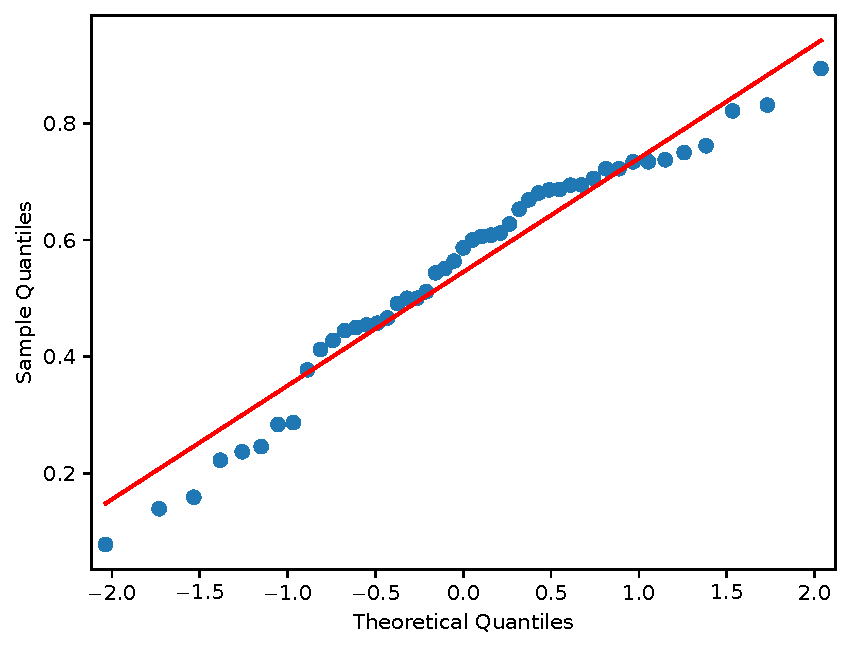
\includegraphics[width=\textwidth]{figs/auc_qqplot_cv.pdf}
        \caption{Q-Q plot over AUC values when training on all datasets except one in one category and testing on the last dataset, aggregated over all categories.}
        \label{fig:strat_all_all_qq}
    \end{subfigure}
    \caption{Histogram over AUC values when training on all datasets except one in a category and testing on the last dataset}
    \label{fig:strat_all_all}
\end{figure}


\subsubsection{Using stages}
The results from stratifying using cancer stages can be found in \autoref{tab:strat_all_stages}. The mean AUCs, both when only using early stage cancer and only using late stage cancer, were only slightly higher than $0.50$ and the differences were not significant, which suggests that there is no improvement in AUC by stratifying by stage.

\begin{table}
    \caption{The results when training on all datasets except one, using datasets where cancer stage is labeled, when stratifying by cancer stage}
    \label{tab:strat_all_stages}
    \sisetup{round-mode=places, round-precision=3}
    \begin{center}
        \csvreader[head to column names, tabular=|r|c|c|c|c|,
        table head = \hline \bfseries Cancer stage & \bfseries Mean & \bfseries Std. & \bfseries t-value & \bfseries p-value \\\hline,
        late after line=\\, late after last line=\\\hline]{tables/Stratification/auc_merged_stages.csv}{}{
            \csvcoli & \num{\csvcolii} & \num{\csvcoliii} & \num{\csvcoliv} & \num{\csvcolv}
        }
    \end{center}
\end{table}

\section{PCA for removing artifacts}
\label{sec:pca_remove_artifacts_res}
The measured miRNA-levels will have some noise that is due to the technology that is used for measurement. One possible way to remove technical noise is to remove the first two principal components from the data, with an assumption that the removed principal components correspond to technical noise rather than biology. It is difficult to say whether this is the case or not. If the datasets are more comparable when the principal components are removed than when they are not, then it would seem plausible that these principal components correspond to technical noise, or at least have little to no connection with lung cancer.


\subsection{Check comparability using PCA}
One way to check if the datasets are more comparable is to check their joint PCA-plot. There are some problems with that. For once, the miRNA-sequences are not the same in the different datasets, which means that the principal components will not represent the datasets fully. Another problem is that there are many datasets. The more datasets that are plotted in one PCA-plot, the more chaotic the plot becomes, the fewer miRNA-sequences there are in common, and the less weight each dataset would have on the PCA on the joint dataset. On the other hand, I cannot plot all datasets against all datasets, as that would lead to too many PCA-plots. Therefore, I will plot two and two datasets in PCA-plots and see whether they became more comparable, using only the largest datasets.

The resulting PCA-plots when the two first principal components are removed are shown in \autoref{fig:pca_remove_two}. It is hard to say whether the PCA adjustments made the datasets more similar using these PCA-plots, but it seems like the spreads are more equal after the removal of the principal components, with the exception of \citet{Asakura2020} and \citet{Fehlmann2020}.

\begin{pycode}
base_dir = "tables/PCA/RemoveTwo/"
for i, f in enumerate(os.listdir(base_dir + "After")):
    s1, s2 = f.split(".csv")[0].split("_vs_")
    print(r"""\begin{figure}""")
    if i:
        print(r"""\ContinuedFloat""")
    print(r"""\begin{subfigure}[t]{0.48\textwidth}
        \resizebox{\textwidth}{!}{
            \begin{tikzpicture}
                \begin{axis}[
                        xlabel={Principal Component 1},
                        ylabel={Principal Component 2},
                    ]
                    \addplot[
                        scatter,only marks,scatter src=explicit symbolic,
                        scatter/classes={
                                A={green},
                                B={red}
                            },
                        table/col sep=comma,
                        mark size=1pt
                    ]""")
    print("""table[x=PCA1,y=PCA2,meta=Type]{{{2}}};
                    \\legend{{\\citet{{{0}}}, \\citet{{{1}}}}}""".format(s1, s2, base_dir + "Before/" + f))
    print(r"""  \end{axis}
            \end{tikzpicture}
            }""")
    print("""\\caption{{PCA of \\citet{{{0}}} and \\citet{{{1}}} using two the principal components of the joint dataset, without any principal components removed}}
        \\label{{fig:pca_{0}_vs_{1}_before}}""".format(s1, s2))
    print(r"""\end{subfigure}%""")
    print(r"\hspace{0.04\textwidth}%")
    print(r"""\begin{subfigure}[t]{0.48\textwidth}
        \resizebox{\textwidth}{!}{
            \begin{tikzpicture}
                \begin{axis}[
                        xlabel={Principal Component 1},
                        ylabel={Principal Component 2},
                    ]
                    \addplot[
                        scatter,only marks,scatter src=explicit symbolic,
                        scatter/classes={
                                A={green},
                                B={red}
                            },
                        table/col sep=comma,
                        mark size=1pt
                    ]""")
    print("""table[x=PCA1,y=PCA2,meta=Type]{{{2}}};
                    \\legend{{\\citet{{{0}}}, \\citet{{{1}}}}}""".format(s1, s2, base_dir + "After/" + f))
    print(r"""  \end{axis}
            \end{tikzpicture}
            }""")
    print("""\\caption{{PCA of \\citet{{{0}}} and \\citet{{{1}}} using two the principal components of the joint dataset, after the two first principal components of each dataset are removed}}
        \\label{{fig:pca_{0}_vs_{1}_after}}""".format(s1, s2))
    print(r"""\end{subfigure}\end{figure}""")
\end{pycode}
\begin{figure}
\py{"\\ContinuedFloat"}
\caption{PCA of datasets with and without removing the two first principal components in each individual dataset}
\label{fig:pca_remove_two}
\end{figure}

\subsection{Using machine learning models}
The results from combining all datasets using sequencing were relatively good (see \autoref{subsec:res_strat_all_technology}), and will therefore be used to check if removing the principal components lead to better comparability, as you would assume that a dataset where noise is removed would be a dataset that would be more comparable to the sequencing datasets, as the sequencing datasets seem to have some external validity when compared to other sequencing datasets.

The way this will be done is for each dataset that is not using sequencing, I will find the miRNAs that they have in common with all the sequencing datasets. Thereafter, using these miRNAs I will do a leave-one-out cross validation on the sequencing datasets, similarly to \autoref{subsec:res_strat_all}. I will also do a cross validation on the other dataset, similar to \autoref{sec:res_machine_learning_single}. Finally, I will train a model on the other dataset and test on the sequencing datasets, and vice versa. All the machine learning will be done using XGBoost, as it was that model that performed well in \autoref{subsec:res_strat_all_technology}.

The resulting AUC-values from doing the experiment are shown in \autoref{tab:pca_remove_noise_no_pca} and \autoref{tab:pca_remove_noise_pca}. The internal results were poorer both in the sequencing datasets and in the non-sequencing datasets, which means that some information about case-control was lost when removing the two first principal components. This does not mean that these principal components were due to biological factors connected to cancer, it might be technical artifacts like batch effects or be due to demographic differences between cases and controls. The external validity, here represented by to which degree it is possible to get good results when training or testing on sequence data, was low in both cases. Everything considered, the data suggest that removing the two first principal components did not have any effect on the comparability.

\begin{table}
    \caption{The resulting AUC-values when using XGBoost and doing cross validation internally in the given study, doing cross validation inside the sequencing datasets, doing training on the given study and testing in the sequencing datasets, and doing training on the sequencing datasets and testing in the given study, all without removing the two first principal components. \\
    Note: I. = internal, Seq = sequencing, To seq = training model on the study and testing on the sequencing datasets, From seq = training model on the sequencing datasets and testing on the study}
    \label{tab:pca_remove_noise_no_pca}
    \sisetup{round-mode=places, round-precision=3}
    \begin{center}
        \csvreader[head to column names, tabular=|r|c|c|c|c|,
        table head = \hline \bfseries Study & \bfseries I. study & \bfseries I. seq & \bfseries To seq & \bfseries From seq \\\hline,
        late after line=\\, late after last line=\\\hline]{tables/PCACrossValidate/pca_cross_validate_no_pca.csv}{}{
            \ifthenelse{\equal{\csvcoli}{Mean}}{Average}{\citet{\csvcoli}} & \num{\csvcolii} & \num{\csvcoliii} & \num{\csvcoliv} & \num{\csvcolv}
        }
    \end{center}
\end{table}

\begin{table}
    \caption{The resulting AUC-values when using XGBoost and doing cross validation internally in the given study, doing cross validation inside the sequencing datasets, doing training on the given study and testing in the sequencing datasets, and doing training on the sequencing datasets and testing in the given study, all while removing the two first principal components. \\
    Note: I. = internal, Seq = sequencing, To seq = training model on the study and testing on the sequencing datasets, From seq = training model on the sequencing datasets and testing on the study}
    \label{tab:pca_remove_noise_pca}
    \sisetup{round-mode=places, round-precision=3}
    \begin{center}
        \csvreader[head to column names, tabular=|r|c|c|c|c|,
        table head = \hline \bfseries Study & \bfseries I. study & \bfseries I. seq & \bfseries To seq & \bfseries From seq \\\hline,
        late after line=\\, late after last line=\\\hline]{tables/PCACrossValidate/pca_cross_validate_pca.csv}{}{
            \ifthenelse{\equal{\csvcoli}{Mean}}{Average}{\citet{\csvcoli}} & \num{\csvcolii} & \num{\csvcoliii} & \num{\csvcoliv} & \num{\csvcolv}
        }
    \end{center}
\end{table}

\section{Finding RPM threshold for sequencing data}
\label{sec:res_rpm_threshold}
\begin{pycode}
df = pd.read_csv("tables/rpm_threshold_cv.csv", index_col=0)
\end{pycode}
Not all miRNA-sequences are measured in all samples in the sequencing datasets. One question is what to do when a sequence is barely read in a dataset. One might remove it or not, depending on whether one considers the levels of the miRNA-sequence relevant or not. As these sequences are barely read, they might be a source of noise rather than a source of information about case-control characteristics. One way to analyze whether they are noise or they have relevant information is to check the consistency across the sequencing datasets when they are removed and when they are not removed.

Here I have taken leave-one-out cross validation on the sequencing datasets, filtering out low expressed miRNAs at different thresholds for mean RPM, as described in \autoref{sec:met_sequencing_thresholds}. The results are shown in \autoref{tab:auc_sequencing_thresholds}. There are a few things to note. The first thing is that the $0$, $1$ and $10$ thresholds give the same number of miRNAs in the intersection, but still the results differ. This is because the normalization of the data was done after filtering out miRNAs based on RPM. When setting the mean variance to $1$ in a dataset, this will lead to a different denominator depending on which miRNAs were filtered out. Thus, the numerical values differ slightly at the different thresholds, even if the miRNAs in the intersection are the same. Secondly, it is interesting to see that one gets a mean AUC of \py{"$%.3f$" % df.loc[1000, "intersection"]}, with only \py{df.loc[1000, "mirna-intersection"]} different miRNAs, where these miRNAs might be found to predict case-control characteristics well.

\begin{table}
    \caption{The resulting AUC-values when doing the experiment as described in \autoref{sec:met_sequencing_thresholds}. The threshold is the mean RPM needed for a miRNA-sequence to be included in the dataset. Intersection (I) and union (U) represent whether the model was trained on the intersection of the miRNAs (logistic regression) or the union of the miRNAs (XGBoost). \# miRNA is the number of miRNAs in the intersection or the union of the datasets, when filtered according to the thresholds}
    \label{tab:auc_sequencing_thresholds}
    \sisetup{round-mode=places, round-precision=3}
    \begin{center}
        \csvreader[head to column names, tabular=|r|r|r|r|r|,
        table head = \hline \bfseries Threshold & \bfseries AUC (I) & \bfseries \# miRNA (U) & \bfseries AUC (U) & \bfseries \# miRNA (U)\\\hline,
        late after line=\\, late after last line=\\\hline]{tables/rpm_threshold_cv.csv}{}{
            \csvcoli & \num{\csvcolii} & \csvcoliii & \num{\csvcoliv} & \csvcolv
        }
    \end{center}
\end{table}

\begin{pycode}
df2 = pd.read_csv("tables/rpm_threshold_aucs_pvalue.csv")
\end{pycode}

To check whether these \py{df.loc[1000, "mirna-intersection"]} miRNAs actually predict case-control status, I did an experiment where I trained logistic regression models on the 1000 RPM thresholded sequencing datasets using intersection between the \py{df.loc[1000, "mirna-intersection"]} miRNAs and the miRNAs in the different other datasets if there were at least 4 miRNAs in common. I compared that to the same experiment using the non-thresholded sequencing datasets and all miRNAs that were in common between the sequencing datasets and the other datasets, where the models thus generally could use more miRNA-sequences. The other datasets were used as test sets. The results are shown in \autoref{tab:auc_sequencing_thresholds_auc}. There was no significant difference between the experiment when using the thresholded datasets and when using the non-thresholded datasets (\py{"$p=%.3f$" % df2["pvalue"]}). This suggests that either the non-sequencing datasets generally have poor quality or these miRNAs are not as predictive of case-control characteristics as it would seem from looking at results only from the sequencing datasets.

\begin{table}
    \caption{The resulting AUC-values when doing logistic regression training on either the 1000 RPM thresholded or the non-thresholded sequencing datasets, using all miRNAs that the datasets have in common in the respective cases}
    \label{tab:auc_sequencing_thresholds_auc}
\sisetup{round-mode=places, round-precision=3}
    \begin{center}
        \csvreader[head to column names, tabular=|r|r|r|,
        table head = \hline \bfseries Study & \bfseries AUC no threshold & \bfseries AUC threshold \\\hline,
        late after line=\\, late after last line=\\\hline]{tables/rpm_threshold_aucs.csv}{}{
            \ifthenelse{\equal{\csvcoli}{mean}}{Average}{\citet{\csvcoli}} & \num{\csvcolii} & \num{\csvcoliii}
        }
    \end{center}
\end{table}

\section{Checking for red blood cells}
\label{sec:res_red_blood_cells}
One thing that can go wrong when doing experiments where serum and plasma are extracted (see: \autoref{met:blood_fluid}) is that red blood cells might burst, and their contents will then be spread into the serum and plasma. Then one can end up with different miRNA-levels in this serum or plasma, in a way that would make the resulting sample more similar to a typical whole blood sample rather than a plasma or serum sample.

There are ways to trace whether red blood cells appear in the sample or not, as they have a known footprint in miRNA-levels. According to \citet{rbc_mirnas}, two of the most characteristic miRNAs for red blood cells are miR-486-5p and miR-451a. Thus, high levels of these miRNAs would suggest that miRNA from red blood cells are found in the sample. 

Till now, all comparison of data between dataset has been done on standardized data. However, this standardization sets the mean expression for each miRNA to zero, which removes any differences in mean expression between datasets. As a result, I have to use the raw values, but it is hard to compare the values directly between the datasets, as the raw values are found using different technologies and thus are on different scales. 

The way to come around these issues is to find some miRNA-sequences to use as controls that one can calculate the expression of miR-486-5p and miR-451a relative to. In the studies reviewed by \citet{mrna_baseline} miR-16 and miR-93 were the most common ones. Thus, they are the ones I will use here. The reason I chose to use two different miRNA-sequences both for footprint and control is that it will hopefully paint a more accurate picture, and not all datasets have all sequences, therefore having more sequences lead to the possibility of getting more information on more datasets.

\begin{table}
    \caption{The relative expression of miR-486-5p and miR-451a to miR-16 and miR-93 in the different datasets. The values are calculated as $\frac{\text{footprint expression} - \text{control expression}}{\text{control expression}}$. C = control}
    \label{tab:relative_expression}
\begin{pycode}
df = pd.read_csv("tables/RedBloodCells/relative_expression.csv", index_col=0, keep_default_na=False)
print(r"\begin{tabular}{|r|r|r|r|r|}")
print(r"\hline")
print(r"\bfseries Studies")
for c in df.columns:
    c = list(map(lambda x: x[4:], c.split("_vs_")))
    c[1] = "C: " + c[1]
    k = r" \\ "
    print(f" & \\bfseries \\thead{{{k.join(c)}}}")
print(r"\\ \hline")
for study, row in df.iterrows():
    print(f"\\citet{{{study}}} & ") 
    print(" & ".join(map(lambda x: x.replace("%", r"\%"), row)))
    print(r"\\ ")
print(r"\hline \end{tabular}")
\end{pycode}
\end{table}

The relative expression of miR-486-5p and miR-451a is in \autoref{tab:relative_expression}. There is a lot of variation between the datasets. One interesting experiment is to group them by what blood fraction is used and then take the average, to see whether blood fraction actually matters. As miR-451a with miR-93 as control is the one with the most values, it is the one that will be used. A table of the mean for each blood fraction group is found in \autoref{tab:relative_expression_body_fluid}. Surprisingly, whole blood seemingly has less miR-451a than either the serum or the plasma group. This renders this experiment somewhat meaningless, as miR-451a was meant to find samples with a high level of red blood cells.

\begin{table}
    \caption{The relative expression of miR-451a to miR-93 (with similar formula as in \autoref{tab:relative_expression}). It is the mean when grouped by body fluid. P. Blood = Peripheral blood, Ex = exosomal}
    \label{tab:relative_expression_body_fluid}
    \begin{center}
        \csvreader[head to column names, tabular=|r|r|,
        table head = \hline \bfseries Body fluid & \bfseries Mean \\\hline,
        late after line=\\, late after last line=\\\hline]{tables/RedBloodCells/relative_expression_body_fluid.csv}{}{
            \csvcoli & \csvcolii \%
        }
    \end{center}
\end{table}

\begin{pycode}
df = pd.read_csv("tables/RedBloodCells/relative_variance.csv", index_col=0)
df_whole_blood = df.loc[["Fehlmann2020", "Leidinger2011", "Patnaik2012", "Patnaik2017"], :]
\end{pycode}

Another way to look at it is to see to which degree miR-486-5p and miR-451a vary internally in a dataset. Intuitively, if there are many red blood cells in the dataset, there will be more variance in these miRNAs, as the red blood cells are a main contributor to the level of expression of these miRNAs. A table with the relative variances is in \autoref{tab:relative_variance}. It is interesting to see that \citet{Qu2017} is an outlier in having a high variance in miR-451a as it was more similar to whole blood datasets in \autoref{fig:auc_pca}. Whole blood datasets had the highest relative variance in miR-486-5p but not in miR-451a according to \autoref{tab:relative_variance_body_fluid}. Furthermore, the high relative variance in miR-486-5p in whole blood is largely driven by \citet{Leidinger2014}, which was a big outlier in \autoref{tab:relative_variance}. Excluding \citet{Leidinger2014} gives a mean relative variance in the whole blood datasets of \py{"$%.3f$" % df_whole_blood["hsa-miR-486-5p"].mean()} in miR-486-5p and \py{"$%.3f$" % df_whole_blood["hsa-miR-451a"].mean()} in miR-451a, which are lower even though it is still the highest for miR-486-5p. Given the earlier results and the uncertainty around the current results, it is hard to say whether relative variance has any external validity when it comes to whether samples are contaminated.


\begin{table}
    \caption{The relative variance of miR-486-5p and miR-451a in the different datasets. The relative variance is the variance in the expression of these miRNAs, divided by the mean variance among all miRNAs.}
    \label{tab:relative_variance}
    \sisetup{round-mode=places, round-precision=3}
    \begin{center}
        \csvreader[head to column names, tabular=|r|r|r|,
        table head = \hline \bfseries Study & \bfseries miR-486-5p & \bfseries miR-451a \\\hline,
        late after line=\\, late after last line=\\\hline]{tables/RedBloodCells/relative_variance.csv}{}{
            \citet{\csvcoli} & \ifthenelse{\equal{\csvcolii}{}}{}{\num{\csvcolii}} & \ifthenelse{\equal{\csvcoliii}{}}{}{\num{\csvcoliii}}
        }
    \end{center}
\end{table}

\begin{table}
    \caption{The mean relative variance of miR-486-5p and miR-451a in the datasets in the different groups. The relative variance is the variance in the expression of these miRNAs, divided by the mean variance among all miRNAs. \\
    Note: P. blood = Peripheral blood, Ex = exosomal}
    \label{tab:relative_variance_body_fluid}
    \sisetup{round-mode=places, round-precision=3}
    \begin{center}
        \csvreader[head to column names, tabular=|r|r|r|,
        table head = \hline \bfseries Group & \bfseries miR-486-5p & \bfseries miR-451a \\\hline,
        late after line=\\, late after last line=\\\hline]{tables/RedBloodCells/relative_variance_body_fluid.csv}{}{
            \csvcoli & \ifthenelse{\equal{\csvcolii}{}}{}{\num{\csvcolii}} & \ifthenelse{\equal{\csvcoliii}{}}{}{\num{\csvcoliii}}
        }
    \end{center}
\end{table}

A final way to look at it is to see whether there are many outliers in miR-486-5p or miR-541a expression. One might assume that the expressions of the miRNAs are normally distributed. In that case, one can fit a t-distribution to the data and see whether 95\% of the data is inside the interval where 95\% of the data should lie given by the mean and the standard deviation of the data (see \autoref{subsec:back_interval_t} for how to compute such an interval). The portion in each dataset that is inside such an interval is shown in \autoref{tab:relative_expression_interval}. The dataset with the lowest portion of samples inside the interval was \citet{Leidinger2014}, which also had the highest relative variance of these miRNAs in \autoref{tab:relative_variance}. However, \citet{Leidinger2014} is a whole blood-dataset, so neither the high variance nor the relatively high portions of outliers are due to contamination of red blood cells.

\begin{table}
    \caption{The portion of the samples which has an expression of the given miRNAs inside a 95\% interval given by the sample mean and standard deviation, calculated as in \autoref{subsec:back_interval_t}.}
    \label{tab:relative_expression_interval}
    \sisetup{round-mode=places, round-precision=3}
    \begin{center}
        \csvreader[head to column names, tabular=|r|r|r|,
        table head = \hline \bfseries Study & \bfseries miR-486-5p & \bfseries miR-451a \\\hline,
        late after line=\\, late after last line=\\\hline]{tables/RedBloodCells/relative_expression_interval.csv}{}{
            \citet{\csvcoli} & \ifthenelse{\equal{\csvcolii}{}}{}{\num{\csvcolii}} & \ifthenelse{\equal{\csvcoliii}{}}{}{\num{\csvcoliii}}
        }
    \end{center}
\end{table}


\section{Web application for visualizing data}
\label{sec:res_web_application}
A web application was made in this project in order to make it possible to visualize the data that has been collected.

\subsection{Some considerations that were made during the project}
How should computations, especially computationally expensive computations like PCA, be done? There were three main options:
\begin{enumerate}
    \item Precompute all possible computations
    \item Do computations server-side on demand
    \item Do computations client-side on demand
\end{enumerate}
All three options had their advantages and disadvantages. The main advantage of precomputing all possible computations was to save computation time during the use of the application. One disadvantage was that very many computations had to be done despite the results might not being used. There is also a large amount of resulting data that has to be stored. Another disadvantage that it shares with the ``compute server-side on demand'' is that new data has to be fetched when the user wants to visualize a new result. Finally, one disadvantage of the ``client-side on demand'' is that the raw data files (especially of \citet{Asakura2020}) are quite large. Thus, having to load those before the application can start leads to a long loading time for the application. I tried both the ``precompute'' and the ``client-side'' options, and decided in favor of the ``precompute''-option as it had a low loading time when one visits the web application, and empirically it was on average faster to fetch new results than to compute them client-side, with the biggest difference when doing heavy computations (like PCA) on large datasets (like \citet{Asakura2020}).

Thus all results shown in the dashboard have been precomputed using Python scripts and stored in JSON-files that are loaded into the application on demand.

\subsection{PCA Single Dataset}

The first module that was made for this web application was a module for visualizing the PCA plot for a single dataset. The possible options are (1) to select the dataset whose PCA plot is shown, (2) the principal component for the x-axis, (3) the principal component for the y-axis, (4) the size of the markers (i.e. the dots in the chart representing each sample), (5) the opacity of the markers and (6) whether to color cancer samples differently from control samples. The proportion of variance explained by the principal components is shown in the axis labels.

\subsection{PCA Two Datasets}

Similar to \textit{PCA Single Dataset} with the difference that you also select a second dataset to be plotted. You can also select whether the principal components are computed using only the first dataset, only the second dataset or both datasets. In any way, all the computations only use the miRNAs that are in both datasets. 

\subsection{PCA Two Datasets (Matrix)}

\begin{figure}
    \centering
    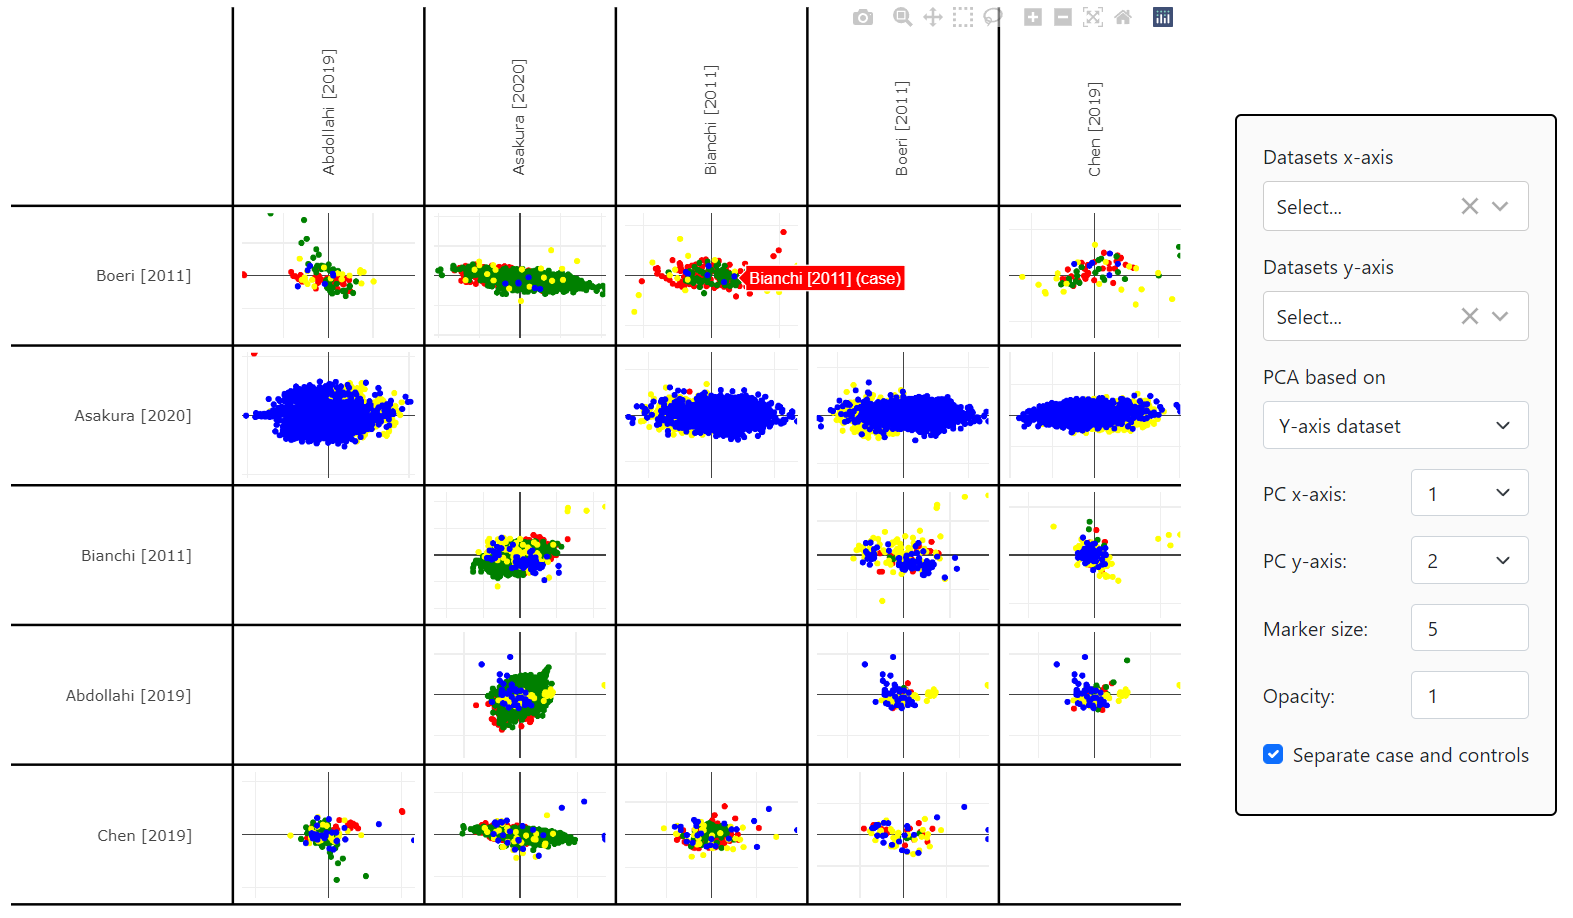
\includegraphics[width=\textwidth]{figs/webapp_screenshots/pca_matrix.png}
    \caption{Screenshot of \textit{PCA Two Datasets (Matrix)}}
    \label{fig:pca_matrix}
\end{figure}

Here, there are several rows and several columns, where each row and each column represents a single dataset. In the intersection between a row and a column, there is a PCA plot similar to \textit{PCA Two Datasets} using the pair of datasets represented by the row and the column. The controls are similar to \textit{PCA Two Dataset}, with the difference that here one selects subsets of datasets to be represented by the rows and the columns respectively. In addition, one selects whether the principal components are calculated based on the row-dataset, the column-dataset or both. Similar to \textit{PCA Two Datasets}, all computations only use the miRNAs that are in both datasets (here: both the column-dataset and the row-dataset). A screenshot is shown in \autoref{fig:pca_matrix}.

\subsection{Boxplot}

\begin{figure}
    \centering
    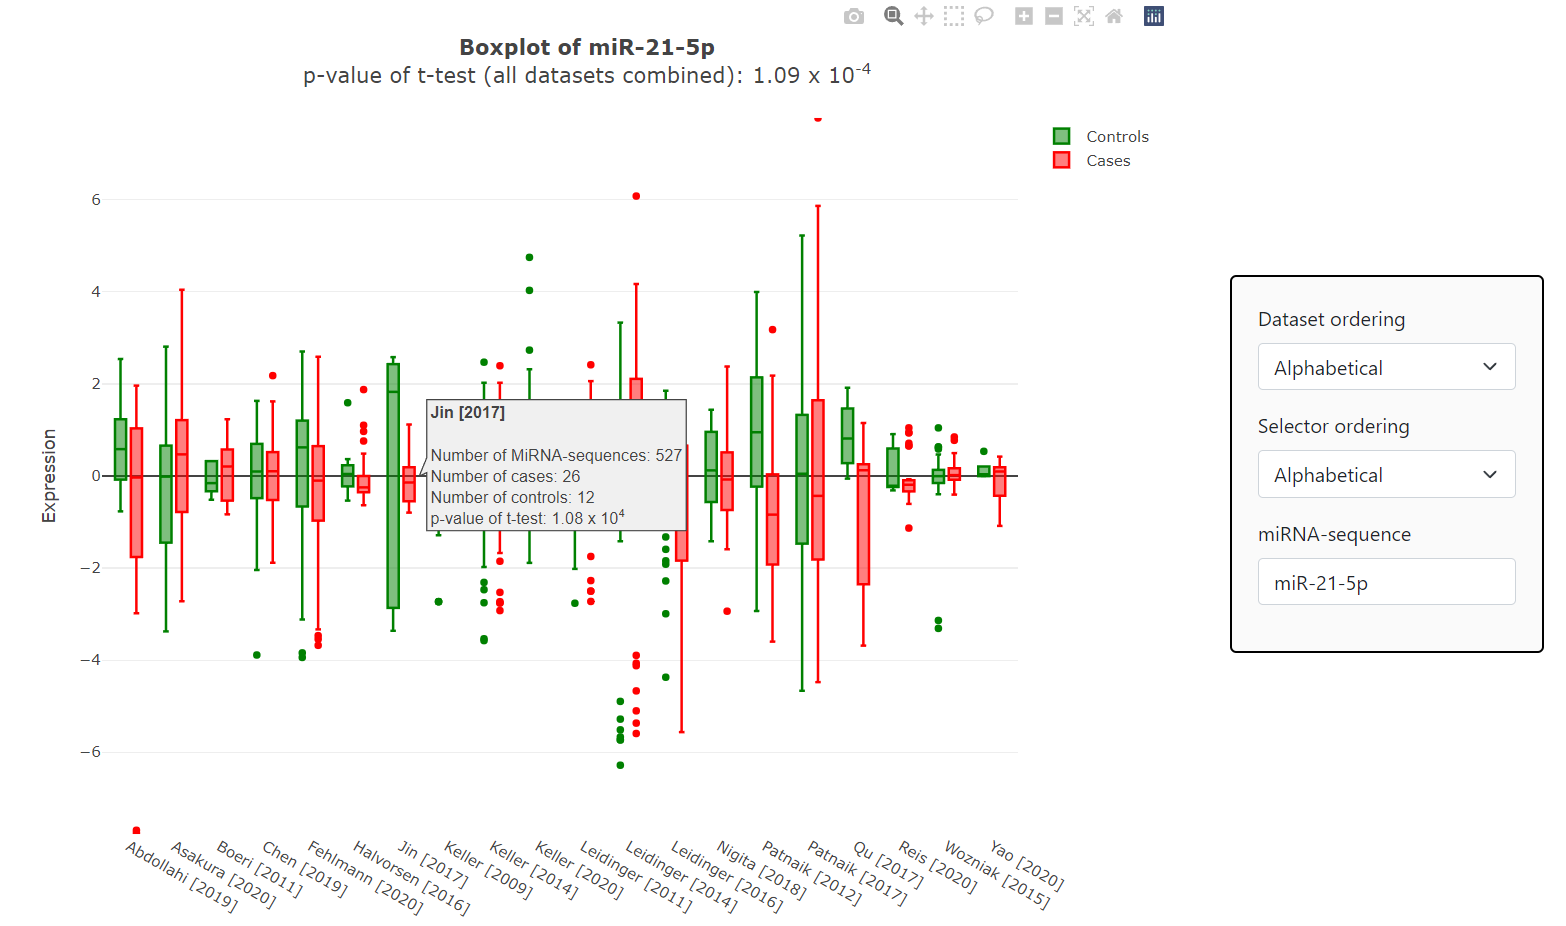
\includegraphics[width=\textwidth]{figs/webapp_screenshots/boxplot.png}
    \caption{Screenshot of \textit{Boxplot}}
    \label{fig:boxplot}
\end{figure}

The boxplot is a plot that shows the expression of a certain miRNA in the different datasets in cases and controls. In addition, a p-value is computed for the separation between cases and controls using a t-test. The p-value is adjusted using Bonferroni, where the p-value for a miRNA-sequence is multiplied by the number of miRNA-sequences and the p-value for a single combination of miRNA and dataset is multiplied by the number of miRNA and dataset combinations. There are three options here: (1) the ordering of the datasets in the boxplot, where one can sort the datasets alphabetically or on either the size or p-value of the separation between cases and controls, (2) the ordering of the miRNA selector (i.e. (3)), where one can either sort the miRNAs alphabetically or based on the p-value of the separation when using all datasets, and finally (3) a selector where one can choose what miRNA will be shown in the boxplot. A screenshot of the boxplot is shown in \autoref{fig:boxplot}.

\subsection{Log Fold Change correlation}

\begin{figure}
    \centering
    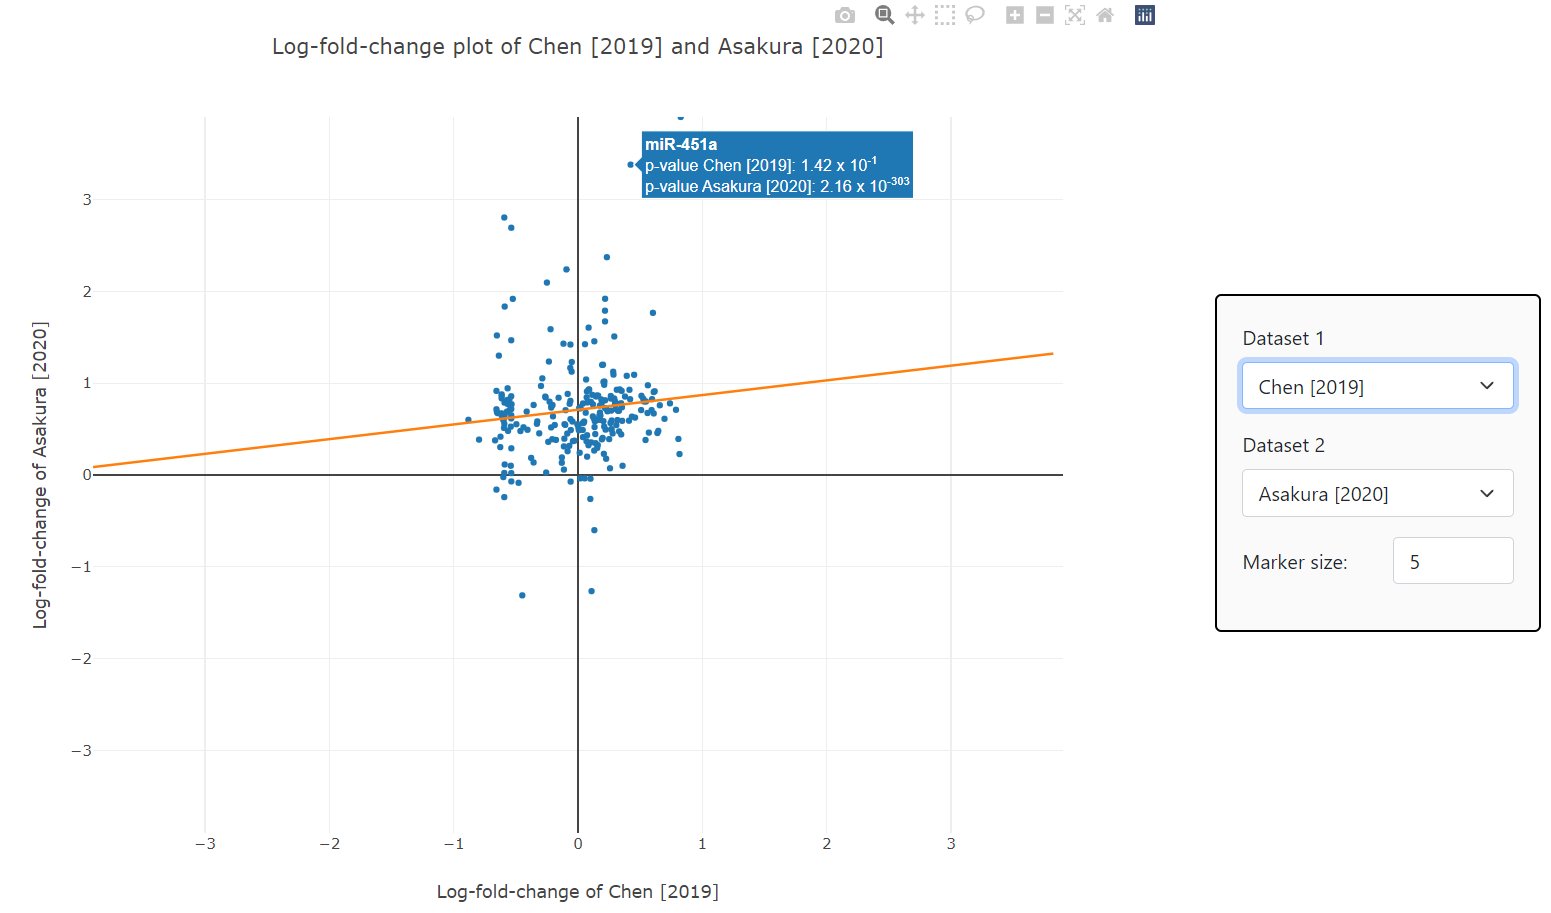
\includegraphics[width=\textwidth]{figs/webapp_screenshots/log_fold_change.png}
    \caption{Screenshot of \textit{Log Fold Change correlation plot}}
    \label{fig:log_fold_change}
\end{figure}

The log fold change correlation plot is a plot where each data point in a scatterplot is the log fold change of a miRNA-sequence in two datasets, where the x-coordinate is the log fold change in the first dataset and the y-coordinate is the log fold change in the second dataset. Each data point is labeled with the miRNA-sequence of the data point and the p-value of the separation between cases and controls in the two datasets using a t-test. There is also a regression line, which is labeled with the correlation in log fold change, and the p-value of the correlation. The options here are (1) to select the two datasets for the plot and (2) the size of the markers. A screenshot of the log fold change correlation plot is shown in \autoref{fig:log_fold_change}.

\subsection{Log Fold Change correlation (Matrix)}

This is a matrix of \textit{Log Fold Change correlation} plots, made in a similar manner to \textit{PCA Two Datasets (Matrix)} as shown in \autoref{fig:pca_matrix}. Here the options are similar to \textit{Log Fold Change correlation}, with the difference that here one can select two subsets of the datasets to be represented by the columns and by the rows respectively.

\subsection{Pairwise machine learning}
The point of this page is to show how well a machine learning algorithm can generalize across two datasets. However, one needs a baseline to compare a model to when assessing how well a machine learning model performs on a task. \Autoref{sec:res_machine_learning_single} shows that a machine learning model generally performs well internally in a dataset, whilst \autoref{sec:res_machine_learning_multiple} shows that a machine learning model generally performs poorly across datasets. 

Comparing an internal machine learning model with a machine learning model across studies might be a good comparison. This is because the internal machine learning model gives a lower bound on how well it is possible to separate cases and controls in a dataset. However, it is not in any way a perfect bound as (1) the internal model might use miRNA expression patterns that are correlated with case-control characteristics in the dataset, but are due to other factors than case-control characteristics and are thus impossible to replicate in other datasets and (2) there might be other patterns of case-control characteristics that an internal model might not recognize due to low sample size, but if these patterns are also present in larger datasets, then a model trained on a larger dataset might outperform the internal model. Anyway, a suboptimal baseline was considered better than none in this case.

The plot is a bar plot of AUC values resulting from training a machine learning algorithm on one of the datasets in a pair of datasets, and then either testing on the same dataset or the other dataset in the pair. The calculation and the meaning of the AUC values in this plot are explained in detail in \autoref{subsec:pairwise_machine_learning_met}. The options here are (1) which pair of datasets to use and (2) what machine learning algorithm to use (with the options: logistic regression, SVM, random forest and XGBoost).

\subsection{Pairwise machine learning (Matrix)}

This is a plot with a matrix of \textit{Pairwise machine learning} plots, made in a similar manner to \textit{PCA Two Datasets (Matrix)}. The options are similar to \textit{Pairwise machine learning}, with the difference that one selects two subsets of the dataset to be represented by the rows and the columns respectively instead of only selecting a pair of datasets.

\subsection{Sample p-value PCA (single)}

One important question is how to identify outlier samples, as outlier samples might be the result of e.g. technical issues, which would mean that removal of these samples would lead to better results. One way is to see how the models classify a certain sample. If the sample has a similar classification pattern as other samples it would be reasonable to assume that the sample is not an outlier. The way I am going to do this is by first taking a dataset as a test set. Then I would find all datasets that have at least four miRNA in common with the test dataset. These datasets would be used as training sets. Each training set is then used for training a machine learning model. The model will then give a probability that each sample in the test set is a cancer sample.

After the probability is calculated for each sample in a test set using each of the training datasets, PCA is conducted on these probabilities.

The machine learning models used here are logistic regression, SVM, random forest and XGBoost; and the whole experiment is conducted once with each of these models.

The proportion of variance explained by the principal components is shown in the axis labels. One can choose to see the PCA loadings, which in this case are the eigenvectors of the PCA. There have been no adjustments on the eigenvectors based on the variance explained. The options are (1) whose test dataset's PCA is shown, (2) whose datasets' loadings are shown, (3) which machine learning algorithm is used, (4) which principal components are plotted along the axes, (5) a scaling for the loadings (as the loadings are unadjusted one might want some scalar scaling as it would change the vector lengths in the plot), (6) marker size, (7) marker opacity, (8) option of whether samples should be shown in the plot and (9) whether to color case and control samples differently. A screenshot of this plot is shown in \autoref{fig:sample_pvalue_pca_single_asakura}.

\subsection{Sample p-value PCA (combined)}
\label{subsec:res_sample_pvalue_combined}
This is similar to \textit{Sample p-value PCA (single)} with the difference that here the PCA is calculated over all samples in all studies. This results in some issues. First of all, the set of training sets can be different for each test set, as it varies which datasets a certain dataset has at least four miRNAs in common with. This is solved by naively setting all probabilities to $0.50$ if the training set does not have at least four miRNAs in common with the test set. Another issue is that the test set also has to be a part of the training sets, as all samples across the datasets are supposed to have the same types of probabilities. This is also naively solved by training and testing on the same dataset. The disadvantage here is that the sample is tested on a model that the sample did also train. Other methods would be to set the prediction probabilities to $0.50$ in that case, with the disadvantage of information getting lost. A last method would be to use some kind of internal cross validation to find a probability, but the disadvantage is that the probability would be calculated in a different way, which would make the numbers less comparable across the datasets.

The plot and the options are similar to \textit{Sample p-value PCA (single)}, with some differences. One difference is that several datasets can be plotted at once (as here the PCA values are comparable across test datasets). Thus, one selects a subset of datasets to be plotted instead of a single dataset. Selecting no datasets is an option, which means that the ``show cases''-option is removed as it is redundant.

\subsection{AUC PCA}
One final question is whether there are any patterns in model performance in a certain test set. One way to check this is to do PCA on the AUC values from testing on a certain dataset while training on all other datasets. Here also, I only train on a dataset if it has at least four miRNAs in common with the test dataset. Thus, the same problem arose as in \textit{Sample p-value PCA (combined)}, with the solution here that I sat $0.50$ as the AUC if the datasets did not have four miRNAs in common. If the training and test datasets were the same I did a $\min(5, \text{\#cases}, \text{\#controls})$-fold cross validation and used the mean AUC.

The plot is similar to \textit{Sample p-value PCA (combined)}, with the difference that the markers represent different datasets rather than samples. In addition, there is an option for choosing a color coding for the markers. The options are no color coding, color the datasets based on technology used (e.g. qRT-PCR, microarray or sequencing) or color the datasets based on the blood fraction where the miRNA-levels were measured (e.g. whole blood, serum or plasma). There is also an option that toggles whether there is a label with the corresponding dataset name near each marker. A screenshot is shown in \autoref{fig:auc_pca}.

\subsection{Pairwise Multi Plot}


In some cases, it might be an advantage to be able to compare two datasets. There are three different ways to compare two datasets in this web application, namely: \textit{PCA Two Datasets}, \textit{Log Fold Change correlation} and \textit{Pairwise Machine Learning}. This plot is a 2x2-matrix with those three plots as subplots. The options here are (1) the pair of datasets; (2) the machine learning algorithm (for \textit{Pairwise Machine Learning}); (3) whether the PCA is based on the first, the second or both datasets; (4) which principal components are plotted; (5) marker size; (6) marker opacity (for \textit{PCA Two Datasets}) and (7) whether to have different colors for cases and controls (for \textit{PCA Two Datasets}).

\section{Results from web application}
\label{sec:res_results_from_web}
The web application allowed for doing analysis with less effort than would otherwise be required. As such, there were also some results from using the web application.

\subsection{Sample p-values PCA (single)}

In general, the models performed poorly when trying to predict across studies, with mean AUCs close to $0.5$. However, by doing PCA on the prediction probabilities one found that the cases and controls differed in how they were predicted by the different models. Here, I want to focus on one example, \citet{Asakura2020}, but other datasets show similar patterns.

\begin{figure}
    \centering
    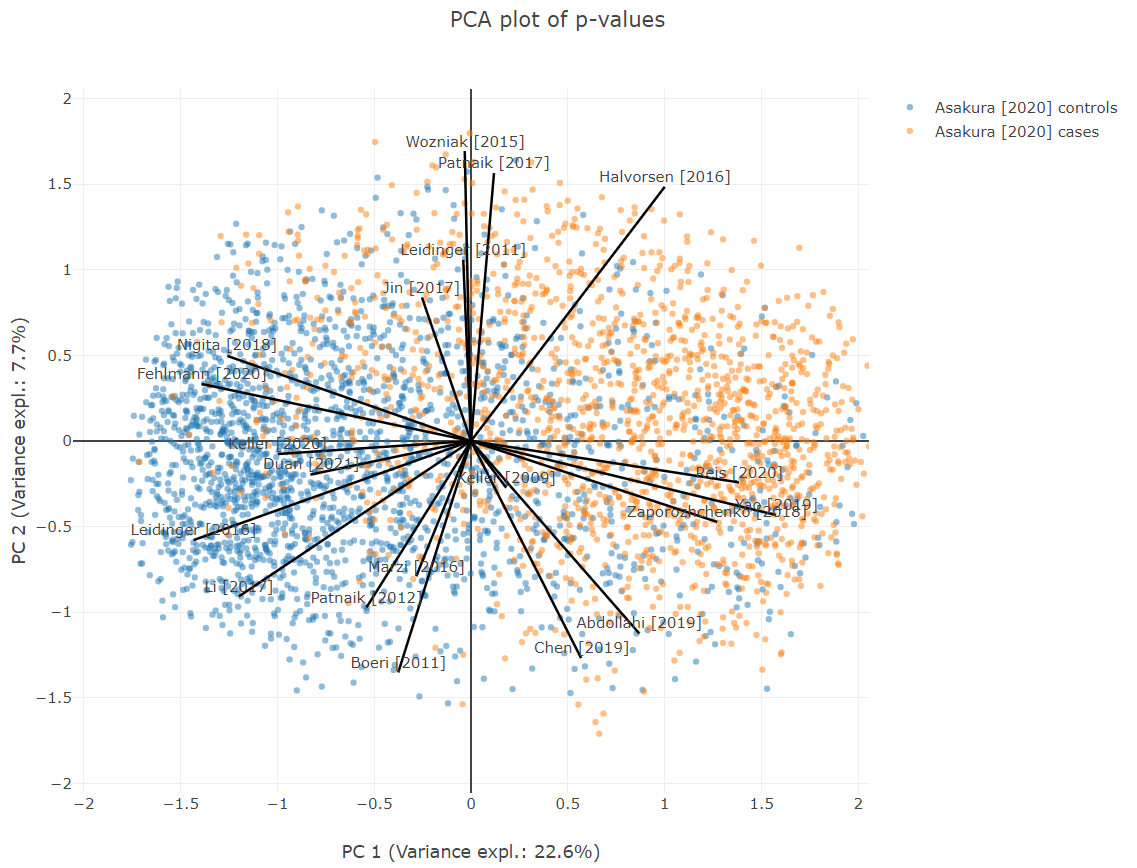
\includegraphics[width=\textwidth]{figs/webapp_screenshots/sample_pvalue_pca_single_asakura.png}
    \caption{Screenshot of \textit{Sample p-value PCA (single)} using \citet{Asakura2020} and logistic regression}
    \label{fig:sample_pvalue_pca_single_asakura}
\end{figure}

The plot is shown in \autoref{fig:sample_pvalue_pca_single_asakura}. Two immediate observations would be:
\begin{enumerate}
    \item The cases and controls are separable in the PCA plot
    \item The loadings are going in very different directions
\end{enumerate}

The first point is somewhat surprising, because as the mean AUC is around $0.50$ one would assume that the models would not be able to separate cases from controls, but the plot suggests that the first principal component (which explains the plurality of the variance in the prediction probability) is at least partially due to case-control characteristics. In other words, despite the models doing no better than chance at predicting cancer status, cancer status is a main contributor to the variance in the predictions of the models.

The second point explains how this can be the case. We see in the plot that giving a high prediction probability from e.g. \citet{Yao2019} or \citet{Reis2020} leads to a high value along PC 1. On the other hand, a high prediction probability from e.g. \citet{Leidinger2016} or \citet{Fehlmann2020} leads to a low value along PC 1. As cases are generally high along PC 1, this means that one would believe that \citet{Yao2019} and \citet{Reis2020} are predicting well, while \citet{Leidinger2016} and \citet{Fehlmann2020} are predicting very poorly as they give high probabilities to controls along PC 1. In aggregate these differences even out as there is little bias for loadings along PC 1, which lead to a mean AUC of $0.50$. Thus the poor results in aggregate hide differences in how the models predict when trained on different datasets. One interesting result would be the correlations in prediction probabilities across studies.

\begin{sidewaystable}
    \caption{The correlation between the prediction probabilities when training on the different datasets given by the column and row names and testing in \citet{Asakura2020} using logistic regression. In addition, the correlation with case status is calculated (i.e. $1$ for cancer, $0$ for control). Green or red color means significant (positive and negative, respectively) correction at a 0.05 level with Bonferroni correction}
    \label{tab:asakura_predictions_correlation}
\begin{pycode}

import pickle
with open("tables/asakura_predictions_correlation.pickle", "rb") as f:
    data = pickle.load(f)

data["studies"].append("Case status")
print("\\resizebox{\\textwidth}{!}{")
print(f"\\begin{{tabular}}{{{'|'.join('r' for _ in data['studies'] + [1])}}} & ")
print(" & ".join("\\multicolumn{1}{c}{\\rotatebox{90}{" + (f"\\citet{{{study}}}" if study != data["studies"][-1] else study) + "}}" for study in data["studies"]))
print("\\\\\hline")
for i, study in enumerate(data["studies"]):
    if i != len(data["studies"]) - 1:
        print(f"\\citet{{{study}}} & ")
    else:
        print(f"{study} & ")
    print(" & ".join((f"\\cellcolor{{{'caribbeangreen' if r > 0 else 'candypink'}}} " if p < 0.05 else "") + ("$%.2f$" % r) for r, p in zip(data["correlation"][i], data["pvalues"][i])))
    print("\\\\")
print("\\end{tabular}}")
\end{pycode}
\end{sidewaystable}

The correlations are plotted in \autoref{tab:asakura_predictions_correlation}. There is little correlation between the predictions from the models trained on \citet{Reis2020} and \citet{Yao2019}. And while \citet{Reis2020} had a large positive correlation with case-characteristics, \citet{Yao2019} had a slight negative correlation. There was a slight negative correlation between the predictions of \citet{Leidinger2016} and \citet{Fehlmann2020}, and while \citet{Leidinger2016} had a slight negative correlation with case status, \citet{Fehlmann2020} had a moderate positive correlation. Thus, even though cases and controls separate well along PC 1, it is important to remember that PC 1 only explains $22.6\%$ of the variance in predictions. The results from the correlation table indeed show that other factors dominate as e.g. \citet{Fehlmann2020} performed moderately well in its predictions overall, even though it predicts in the wrong direction along PC 1. Thus, even though cases and controls separate well along PC 1, this effect almost disappears on an aggregate level as other sources of variance dominate.


%Indeed, there is a significant positive correlation between the predictions from models trained on \citet{Fehlmann2020} and \citet{Yao2019}, and both of their predictions have a significant positive correction with case-control characteristics. On the other hand, the correlation between prediction from models trained on \citet{Leidinger2016} and \citet{Li2017} were poor, and only the predictions from \citet{Li2017} had a significant negative correlation with case control status.

Another interesting observation from the table is that of all the datasets that have been used for training, only the correlations from \citet{Boeri2011}, \citet{Jin2017}, \citet{Keller2020} and \citet{Patnaik2012} were not significant. It is interesting because as the mean AUC was around $0.50$ one might think that predictions were in general independent of case-control characteristics, but this shows that that was not the case. Many datasets have a significant negative correlation with case-control characteristics, which means that there are features in the data that separate cases and controls to some degree, but those features lead the models to predict wrongly. It is difficult to say what is the reason for this. One hypothesis would be that some confounding variables are correlated with case characteristics in one dataset, but are correlated with control characteristics in other datasets. As the Asakura dataset was adjusted for sex and age, either the adjustment using a linear predictor was not sufficient, or the confounding variables are due to other characteristics.

\iffalse
\subsection{Sample p-values PCA (combined)}

The \textit{Sample p-values PCA (combined)} can give some indication of why there are systematic differences in how models predict based on what dataset they are trained on. One can see what loadings between different training sets are similar, which means that they are systematically predicting in the same way. One way to find what models are predicting similarly is to do something like \autoref{tab:asakura_predictions_correlation}, but using all datasets as the test set. The correlation table was made using the same values as calculated in \autoref{subsec:res_sample_pvalue_combined} and is shown in \autoref{tab:predictions_correlation}. One important thing to note is that each test sample is equally weighted, which means that the largest dataset dominate the test set.


\begin{sidewaystable}
    \caption{The correlation between the prediction probabilities when training on the different datasets and testing in all datasets using logistic regression. The column and row names denote the dataset that is used for the training. In addition, the correlation with case status is calculated (i.e. $1$ for cancer, $0$ for control). Green or red color means significant (positive and negative, respectively) correction at a 0.05 level with Bonferroni correction}
    \label{tab:predictions_correlation}
\begin{pycode}

import pickle
with open("tables/predictions_correlation.pickle", "rb") as f:
    data = pickle.load(f)

print("\\resizebox{\\textwidth}{!}{")
studies.append("Case status")
print(f"\\begin{{tabular}}{{{'|'.join('r' for _ in studies + [1])}}} & ")
print(" & ".join("\\multicolumn{1}{c}{\\rotatebox{90}{" + (f"\\citet{{{study}}}" if study != studies[-1] else study) + "}}" for study in studies))
print("\\\\\hline")
for i, study in enumerate(studies):
    if i != len(studies) - 1:
        print(f"\\citet{{{study}}} & ")
    else:
        print(f"{study} & ")
    print(" & ".join((f"\\cellcolor{{{'caribbeangreen' if r > 0 else 'candypink'}}} " if p < 0.05 else "") + ("$%.2f$" % r) for r, p in zip(data["correlation"][i], data["pvalues"][i])))
    print("\\\\")
print("\\end{tabular}}")
studies = studies[:-1]
\end{pycode}
\end{sidewaystable}

I looked at the datasets that correlated best with \citet{Asakura2020} in \autoref{tab:predictions_correlation} using the \textit{Pairwise Multi Plot}. Among the datasets that correlated best with \citet{Asakura2020}, \citet{Patnaik2017} and \citet{Qu2017} had a mean log fold change close to zero, while \citet{Fehlmann2020} and \cite{Reis2020} had a positive mean. This could suggest that some of the correlation in predictions could be due to bias in log fold change as \citet{Asakura2020} also had a positive mean log fold change. The \textit{Pairwise Multi Plot} of \citet{Asakura2020} and \cite{Reis2020} is shown in \autoref{fig:pairwise_multi_plot_asakura_reis}.

% Another thing to note is that the predictions using \citet{Asakura2020} as training set correlate well with predictions using \citet{Reis2020} as a training set. This is also clear from the plot on the web application, as the loadings for \citet{Asakura2020} and \citet{Reis2020} are similar. Using the \textit{Pairwise Multi Plot}, one can compare these two datasets to see why they give similar predictions. A screenshot of this plot is shown in \autoref{fig:pairwise_multi_plot_asakura_reis}.

\begin{figure}
    \centering
    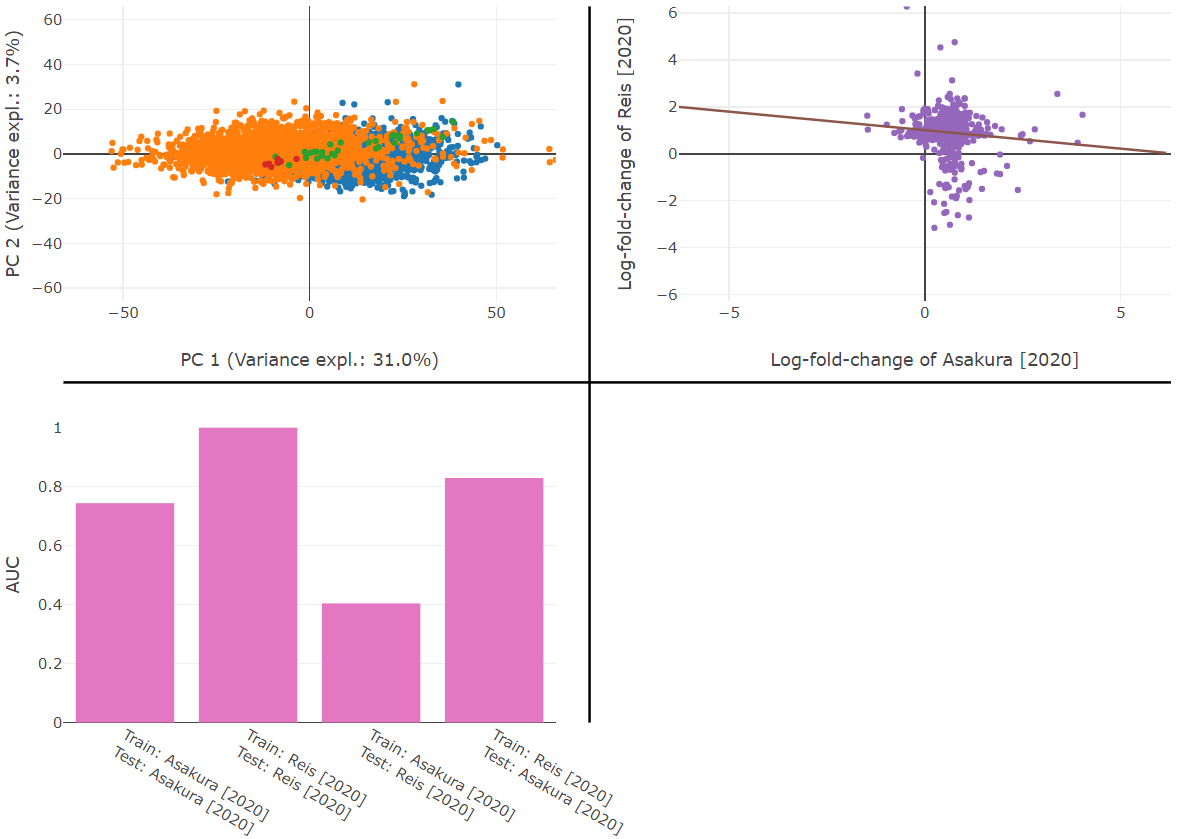
\includegraphics[width=\textwidth]{figs/webapp_screenshots/pairwise_multi_plot_asakura_reis.png}
    \caption{Screenshot of \textit{Pairwise Multi Plot} using \citet{Asakura2020} and \citet{Reis2020}. In the PCA, orange is \citet{Asakura2020} controls, blue is \citet{Asakura2020} cases, red is \citet{Reis2020} controls and green is \citet{Reis2020} cases (this information in shown on hover in the web application)}
    \label{fig:pairwise_multi_plot_asakura_reis}
\end{figure}

% There are several things to note from the multiplot. For once, the separation between cases and controls is going along the first principal component in the same way in both \citet{Asakura2020} and \citet{Reis2020}, which means that there is a separation between cases and controls that are in both datasets, and that contributes to a significant portion of the variance in both datasets. More strikingly, however, is in the log-fold-change plot, where in both datasets miRNAs generally have a larger expression in cases than controls. This might suggest that models trained on \citet{Asakura2020} and \citet{Reis2020} are predicting higher probability for cancer if there is a high level of expression of miRNAs in general. The same phenomena of miRNAs generally being higher expressed in cases is also found in \citet{Duan2021} and to a lesser degree \citet{Fehlmann2020}, which are the datasets with the third and second highest correlations with \citet{Asakura2020} in \autoref{fig:pairwise_multi_plot_asakura_reis} respectively. On the other hand, the dataset with the most negative correlation with \citet{Asakura2020} was \citet{Li2017}, which where miRNAs in general were down-expressed in cases compared with controls.

To check whether it was the case that there was a connection between mean log fold change and the correlations with \citet{Asakura2020}, I did an experiment where I took the corrections with \citet{Asakura2020} in \autoref{tab:predictions_correlation} and the mean log fold change in the different datasets and saw if there was any correlation. The results showed a correlation of \py{"$%.3f$" % data["correlation_asakura"]} which was significantly different from zero with \py{"$p=%.3f$" % data["pvalue_asakura"]}. This suggests that this bias in mean log fold change is partially what leads to correlations in predictions. One question is whether this is noice that should be removed? Or similarly, if this bias in mean log fold change is adjusted for, will the datasets have a higher consistency?

\begin{pycode}
df = pd.read_csv("tables/auc_zero_mean_fold_change.csv")
\end{pycode}

I did an experiment to check whether that was the case. The method was similar to \autoref{subsec:res_strat_two}. I took all pairs of datasets with at least 10 miRNAs in common and then trained a logistic regression model on one dataset and tested on the other dataset. The idea here is that this was twice, one when both datasets were adjusted so that the mean log fold change was zero, and one time without any adjustments. The adjustment was done by subtracting the mean log fold change from all cases, and then re-standardize the dataset so that the overall mean of the dataset would still be zero. This lead to a mean AUC of \py{"$%.3f$" % df["mean (non-zero mean FC)"]} and a standard deviation of \py{"$%.3f$" % df["std (non-zero mean FC)"]} when unadjusted, and a mean of \py{"$%.3f$" % df["mean (zero mean FC)"]} and a standard deviation of \py{"$%.3f$" % df["std (zero mean FC)"]} when adjusted. A two-sided t-test found no significant difference (\py{"$p=%.3f$" % df["p-value"]}). This means that difference mean log fold change was not the only reason that there were poor results when training and testing in pair, and is likely not a main reason for the poor results. It is still possible that the consistency is better when adjusting, but that there are other reasons that AUC values were poor.

Another question that then arises is whether the bias in the mean of the log fold change of all the miRNAs contributes to the covariance in prediction seen in \autoref{tab:predictions_correlation} at all? One way to check this is to check the correlation with and without an adjustment similar to the one in the previous paragraph. The way I will check this is to do a t-test on the difference of $R^2$-values, calculated in a similar way as the values in \autoref{tab:predictions_correlation}, with the difference that I will only calculate correlation based on samples where both datasets have been used to predict the sample. This is because it is the difference in $R^2$-values is what is important here, not that correlations between different pairs of datasets are comparable. The reason for using $R^2$ rather than $r$ is to see whether bias in mean log fold change is a driver of the correlations in predictions, either driving positive or negative correlations. If it indeed is, $R^2$ would be expected to be lower after corrections.



\begin{pycode}
df = pd.read_csv("tables/zero_mean_fold_change_predictions_correlation.csv", index_col=0)
\end{pycode}

The mean $R^2$ when adjusing was \py{"$%.3f$" % df.loc["r2", "mean (zero mean FC)"]} and \py{"$%.3f$" % df.loc["r2", "mean (non-zero mean FC)"]} when not adjusting. Thus, the $R^2$ was significantly higher when adjusted than when not adjusted (\py{"$p=%.3f$" % df.loc["r2", "p-value"]}). It is hard to say from this result, what is the driver of the difference in $R^2$. In particular, is the correlations becoming more positive in general, or is there also more negative correlation? To answer that, one has to do a similar experiment using $r$ instead of $R^2$. If the correlations are becoming more positive in general, it would mean that reducing bias in mean log fold change is one way of data cleaning that leads to better consistency across datasets. I found that the mean $r$ when not adjusting the data was \py{"$%.3f$" % df.loc["r", "mean (non-zero mean FC)"]} and the mean when adjusting the data was \py{"$%.3f$" % df.loc["r", "mean (zero mean FC)"]}, and that the difference was not significant (\py{"$p=%.3f$" % df.loc["r", "p-value"]}). Thus, the correlations were not higher or lower on average, but their magnitudes were higher when adjusting the data. It is difficult to tell what is contributing to this effect.
\fi

\subsection{AUC PCA}

\begin{figure}
    \centering
    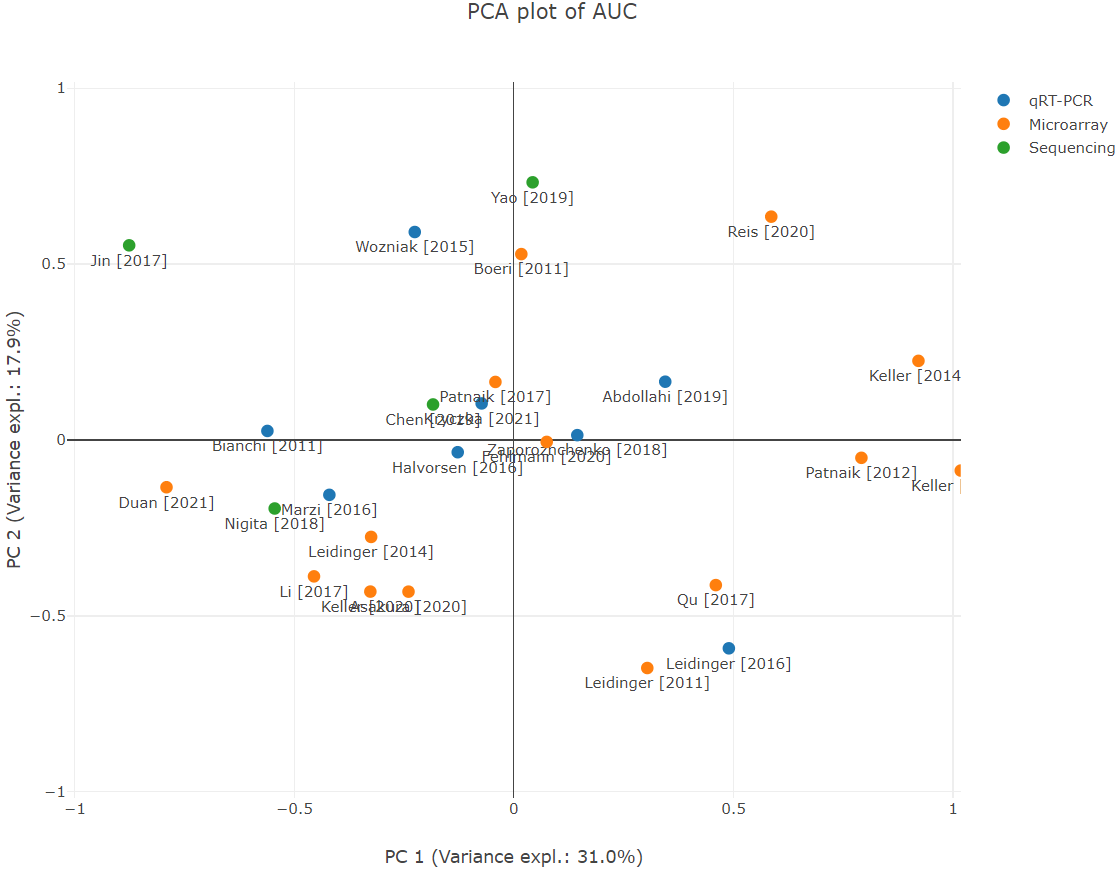
\includegraphics[width=\textwidth]{figs/webapp_screenshots/auc_pca.png}
    \caption{Screenshot of \textit{AUC PCA} when coloring based on technology}
    \label{fig:auc_pca}
\end{figure}
The AUC PCA-plot gave some insight into what created the difference between the datasets. A screenshot is shown in \autoref{fig:auc_pca}, when coloring is based on technology. There is some clustering in the plot based on what technology is used for measuring miRNA-levels. Thus, there is more evidence that heterogeneity in technology is one reason for low consistency across datasets. However, to be sure, it would be useful to do a statistical test to see whether there actually are any differences. In particular, taking a t-test along the first principal component would show whether there actually are any significant differences along that axis.

\begin{pycode}
df = pd.read_csv("tables/auc_pca_t_test.csv", index_col=0)
\end{pycode}

The mean value along the first principal component was \py{"$%.3f$" % df.loc["qRT-PCR_vs_Sequencing", "mean2"]} for the sequencing datasets, \py{"$%.3f$" % df.loc["qRT-PCR_vs_Microarray", "mean1"]} for the qRT-PCR datasets and \py{"$%.3f$" % df.loc["qRT-PCR_vs_Microarray", "mean2"]} for the microarray datasets. The difference between qRT-PCR and microarrays was not significant (\py{"$p=%.3f$" % df.loc["qRT-PCR_vs_Microarray", "p-value"]}). Likewise, the difference between sequencing and microarrays (\py{"$p=%.3f$" % df.loc["Microarray_vs_Sequencing", "p-value"]}), and the difference between qRT-PCR and sequencing (\py{"$p=%.3f$" % df.loc["qRT-PCR_vs_Sequencing", "p-value"]}) were not significant.


\iffalse
\section{Experimental Plan}
\label{sec:experimentalPlan}

Trying and failing is a major part of research. However, to have a chance of success you need a plan driving the experimental research, just as you need a plan for your literature search. Further, plans are made to be revised and this revision ensures that any further decisions made are in line with the work already completed.  

The plan should include what experiments or series of experiments are planned and what question the individual or set of experiments aim to answer. Such questions should be connected to your research questions so that in the evaluation of your results you can discuss the results wrt to the research questions.  

\section{Experimental Setup}
\label{sec:experimentalSetup}

The experimental setup should include all data - parameters etc, that would allow a person to repeat your experiments. 

\section{Experimental Results}
\label{sec:experimentalResults}

Results should be clearly displayed and should provide a suitable representation of your results for the points you wish to make. Graphs should be labeled in a legible font and if more than one result is displayed on the same graph then these should be clearly marked.   Please choose carefully rather than presenting every results. Too much information is hard to read and often hides the key information you wish to present. Make use of statistical methods when presenting results, where possible to strengthen the results.  Further, the format of the presentation of results should be chosen based on what issues in the results you wish to highlight. You may wish to present a subset in the experimental section and provide additional results in the appendix.

\fi
